\documentclass[a4paper, 12pt]{article}
\usepackage[T1]{fontenc}
\usepackage[utf8]{inputenc}
\usepackage[italian]{babel,varioref}
\usepackage{url}
\usepackage{hyperref}
\usepackage{booktabs}
\usepackage{graphicx}
\usepackage{amsmath}
\usepackage{float}

\begin{document}

% FRONTESPIZIO

\begin{titlepage}
	\begin{center}
		\begin{huge}
			\textbf{POLITECNICO DI TORINO}
			
		\end{huge}
		\vspace{0.4cm}
		\begin{large}
			Dipartimento di Ingegneria Gestionale e della Produzione\\
			\vspace{0.3cm}
			\textbf{DIGEP}\\
		\end{large}
		
		\vspace{1.3cm}		
		
		
\includegraphics[width=0.4\textwidth]{IMG/PoliTO_logo.png}
		
		\vspace{1.3cm}
		
		\begin{Large}
		\textbf{Corso di Laurea in Ingegneria Gestionale}\\
		\vspace{0.3cm}
		percorso dell'informazione, classe \textbf{l-8}
		\end{Large}
		
		\vspace{1cm}
		
		\begin{Large}
			Elaborato di Laurea Triennale\\
		\end{Large}
		
		\vspace{0.5cm}
		
		\begin{LARGE}
			\textbf{Quarantine Simulator}\\
		\end{LARGE}
	
		\vspace{0.1cm}
	
		\begin{large}
			un tool per la gestione delle epidemie\\
		\end{large}
	
		\vspace{1cm}
		
	\end{center}

	\textbf{Relatore:} Prof. Fulvio Corno
	\hfill
	\textbf{Studente:} Luca Debernardi
	
	\vfill
	
	\begin{center}
		Periodo di iscrizione: 2017/2020
	\end{center}
	
\end{titlepage}

% INIZIO

\newpage
% PAGINA VUOTA PER FARE SCENA

$\text{}$

\vfill

\begin{center}
	\emph{
	Breve guida introduttiva scritta in \LaTeX{}\\
	della Tesi di Laurea Triennale\\
	"Quarantine Simulator",\\
	Luca Debernardi\\
	S244685\\
	\textbf{.}}
\end{center}

\vspace{3cm}


\title{Quarantine Simulator}

\author{Luca Debernardi - s244685}
\date{Settembre 2020}

\maketitle

\tableofcontents

\listoffigures


\newpage
% PROPOSTA

\section{Proposta}
	\subsection{Titolo}
	
	Quarantine Simulator
	
	\subsection{Problema}
	
	L'obiettivo dell'applicazione è fornire uno strumento utile alla simulazione della diffusione del Coronavirus (o di qualsiasi altro virus) all'interno del territorio italiano.
	Selezionando uno o più punti di partenza, è possibile osservare dove e quando il virus si espande nelle aree limitrofe e quindi studiare efficaci metodi per rallentarne la corsa.
	
	\subsection{Rilevanza gestionale}
	
	Un software come questo, malgrado tutte le ovvie semplificazioni del caso, fornisce uno strumento per simulare lo sviluppo di una pandemia sul territorio nazionale.
	I risultati forniti permettono quindi di analizzare le ripercussioni sulla diffusione in accordo alle decisioni prese, sia a priori, sia in diretta.
	Ovviamente, data la scarsa conoscenza che possediamo del virus, i risultati non sono confrontabili al 100\% con la realtà, ma permettono comunque di comprendere come alcune decisioni possano influenzare in maniera determinante l'evolversi di un'epidemia.
	
	\subsection{Data-set}
	\label{sub:db}
	
	L'applicazione si basa su una versione leggermente modificata (e depurata dagli errori) del dataset Comuni-Province-Regioni italiane 2018, raggiungibile dalla URI:\\
	\url{https://github.com/Debe98/db_Italia}\footnote{Il nome del database, in formato sql, è  \emph{create-database-comuni-italiani-2018.sql}.\\
	L'autore originale, \emph{MatteoHenryChinaski}, è indicato dalla fonte del fork.}\\
	Questo DB offre una valida rappresentazione del territorio italiano, fornendo per ogni comune, provincia e regione dati sulla popolazione, sulla superficie e sulla posizione (come latitudine e longitudine).

	\subsection{Algoritmi}
	
	L'algoritmo cardine è ovviamente quello della simulazione, utilizzata per stimare, giorno per giorno, l'evoluzione della diffusione del virus.
	La difficoltà principale è gestire un grafo di grandi dimensioni: infatti il numero di comuni italiani è all'incirca di 8000 unità (che sarebbero i nodi del nostro grafo); impossibile anche solo immaginare un grafo completo, che comporterebbe l'astronomica cifra di 64 milioni di archi.
	Per risolvere questa problematica sono state attuate due strategie:
	
	\begin{itemize}
		
		\item Definizione di diversi gradi di aggregazione: comunale, provinciale e regionale, ciascuno con le proprie adiacenze e relazioni.
		
		\item Creazione degli archi solo sulla base delle adiacenze.\\
		Questa informazione non è presente nel DB, la strategia con cui sono state ottenute (in modo approssimato ma comunque molto affidabile) verrà spiegata più avanti nella trattazione.
		
		\item Ogni tipologia di ente territoriale ha un grafo proprio, che viene utilizzato con un ruolo diverso a seconda dell'aggregazione scelta dall'utente.
		
	\end{itemize}
	La simulazione, per descrivere l'evoluzione della situazione, deve aggiornare ad ogni iterazione sia tutti i nodi, sia tutte le interazioni tra i nodi vicini (l'arrivo del virus in un comune confinante); la complessità della singola iterazione è quindi O(V+A).
	Il numero di iterazioni dipende sia dall'obiettivo che viene scelto, sia dai parametri che vengono forniti e quindi non è stimabile a priori.\\
	Per maggiori dettagli sulla complessità computazionale, consultare la sezione \vref{sec:log}.
	
	\subsection{Funzionalità}
	
	L'applicazione sarà strutturata secondo la seguente logica:
	
	\begin{itemize}
	
	\item \textbf{Parametri:} tab in cui è possibile modificare i parametri relativi al virus e al mondo. 
	\item \textbf{Simulazione:} tab in cui è possibile regolare le proprie preferenze riguardo alla simulazione.
	\item \textbf{Risultati:} tab in cui è possibile analizzare i risultati sotto forma tabellare e grafica.
	
	\end{itemize}

\newpage
% MOTIVAZIONE

\section{Perché questo argomento?}
	Fin dall'infanzia ho sempre adorato la matematica, una materia teoricamente astratta, ma allo stesso tempo tanto concreta da essere una parte fondamentale di qualsiasi sfumatura delle nostre vite.
	Crescendo, ho imparato che non era tanto la matematica che amavo, quanto la sua incredibile versatilità, che la rendeva lo strumento perfetto per fare ciò che davvero volevo fare: risolvere problemi reali, pratici, concreti.
	Cercare la soluzione di rompicapi ogni volta più complessi è da sempre il mio hobby, la stella polare che mi ha guidato finora e che più di ogni altra mi ha convinto ad iscrivermi qui, al Politecnico di Torino.\\
	La recente pandemia di Coronavirus, che ha colpito duramente non solo il nostro Paese ma tutto il mondo, è stata (e forse continuerà ad essere) con ogni probabilità la più grande sfida che abbiamo dovuto affrontare negli ultimi 50 anni.\\
	Ebbene quale modo migliore di terminare questa prima parte del mio percorso, se non unire tutto ciò che ho imparato in questi anni per aiutare a trovare soluzioni al più grande problema dell'ultimo mezzo secolo?

\newpage
% LEGENDA

\section{Legenda}

	Prima di addentrarci nei meandri della logica applicativa, ritengo opportuno definire una volta per tutte alcune delle nomenclature necessarie per usare il programma al meglio delle sue possibilità:
	
	\subsection{AggregationType}
		Questa enumerazione permette di definire a che tipologia di ente ci stiamo riferendo; la classificazione è abbastanza immediata:
		
		\begin{itemize}
			\item \textbf{COMUNE}
			\item \textbf{PROVINCIA}
			\item \textbf{REGIONE}
		\end{itemize}
	
	\subsection{Status}
		Ogni persona, durante la simulazione, si trova in uno di questi stati. Il passaggio dall'uno all'altro determina l'avanzamento dell'epidemia.
		Gli stati considerati sono: 
		
		\begin{itemize}
			\item \textbf{SANO:} parte di popolazione che ancora non è entrata in contatto con il virus ed è quindi a rischio.
			\item \textbf{CONTAGIOSO:} persone che hanno contratto il virus e sono contagiose, ma che non mostrano ancora alcun sintomo.
			\item \textbf{GUARITO:} stato terminale delle persone che sono guarite dalla malattia da sole (asintomatici).
			\item \textbf{MALATO:} persone che hanno iniziato a mostrare i sintomi.
			In questa simulazione, i malati contano come rimossi (non trasmettono più il virus), in quanto si considerano messi in quarantena o ospedalizzati.\textbf{*}
			\item \textbf{CURATO:} numero di persone che guarisce in modo definitivo.\textbf{*}
			\item \textbf{MORTO:} persone che non riescono a sopravvivere al virus.\textbf{*}
			\item \textbf{FREE:} non è un status a tutti gli effetti, ma l'unione di alcuni dei precedenti. Più specificatamente, indica la popolazione libera di muoversi e quindi di generare contatti.\\
			FREE = \{SANO, CONTAGIOSO, GUARITO, CURATO\}\textbf{*}
		\end{itemize}
		Gli stati contrassegnati con \textbf{*} sono gli unici  per cui è possibile il confronto tra realtà e simulazione.\\
		Il flowchart del cambio di stato è riportato qui sotto, nella figura \vref{fig:stati}.
		
		 \begin{figure}[H]
		 	\centering
		 	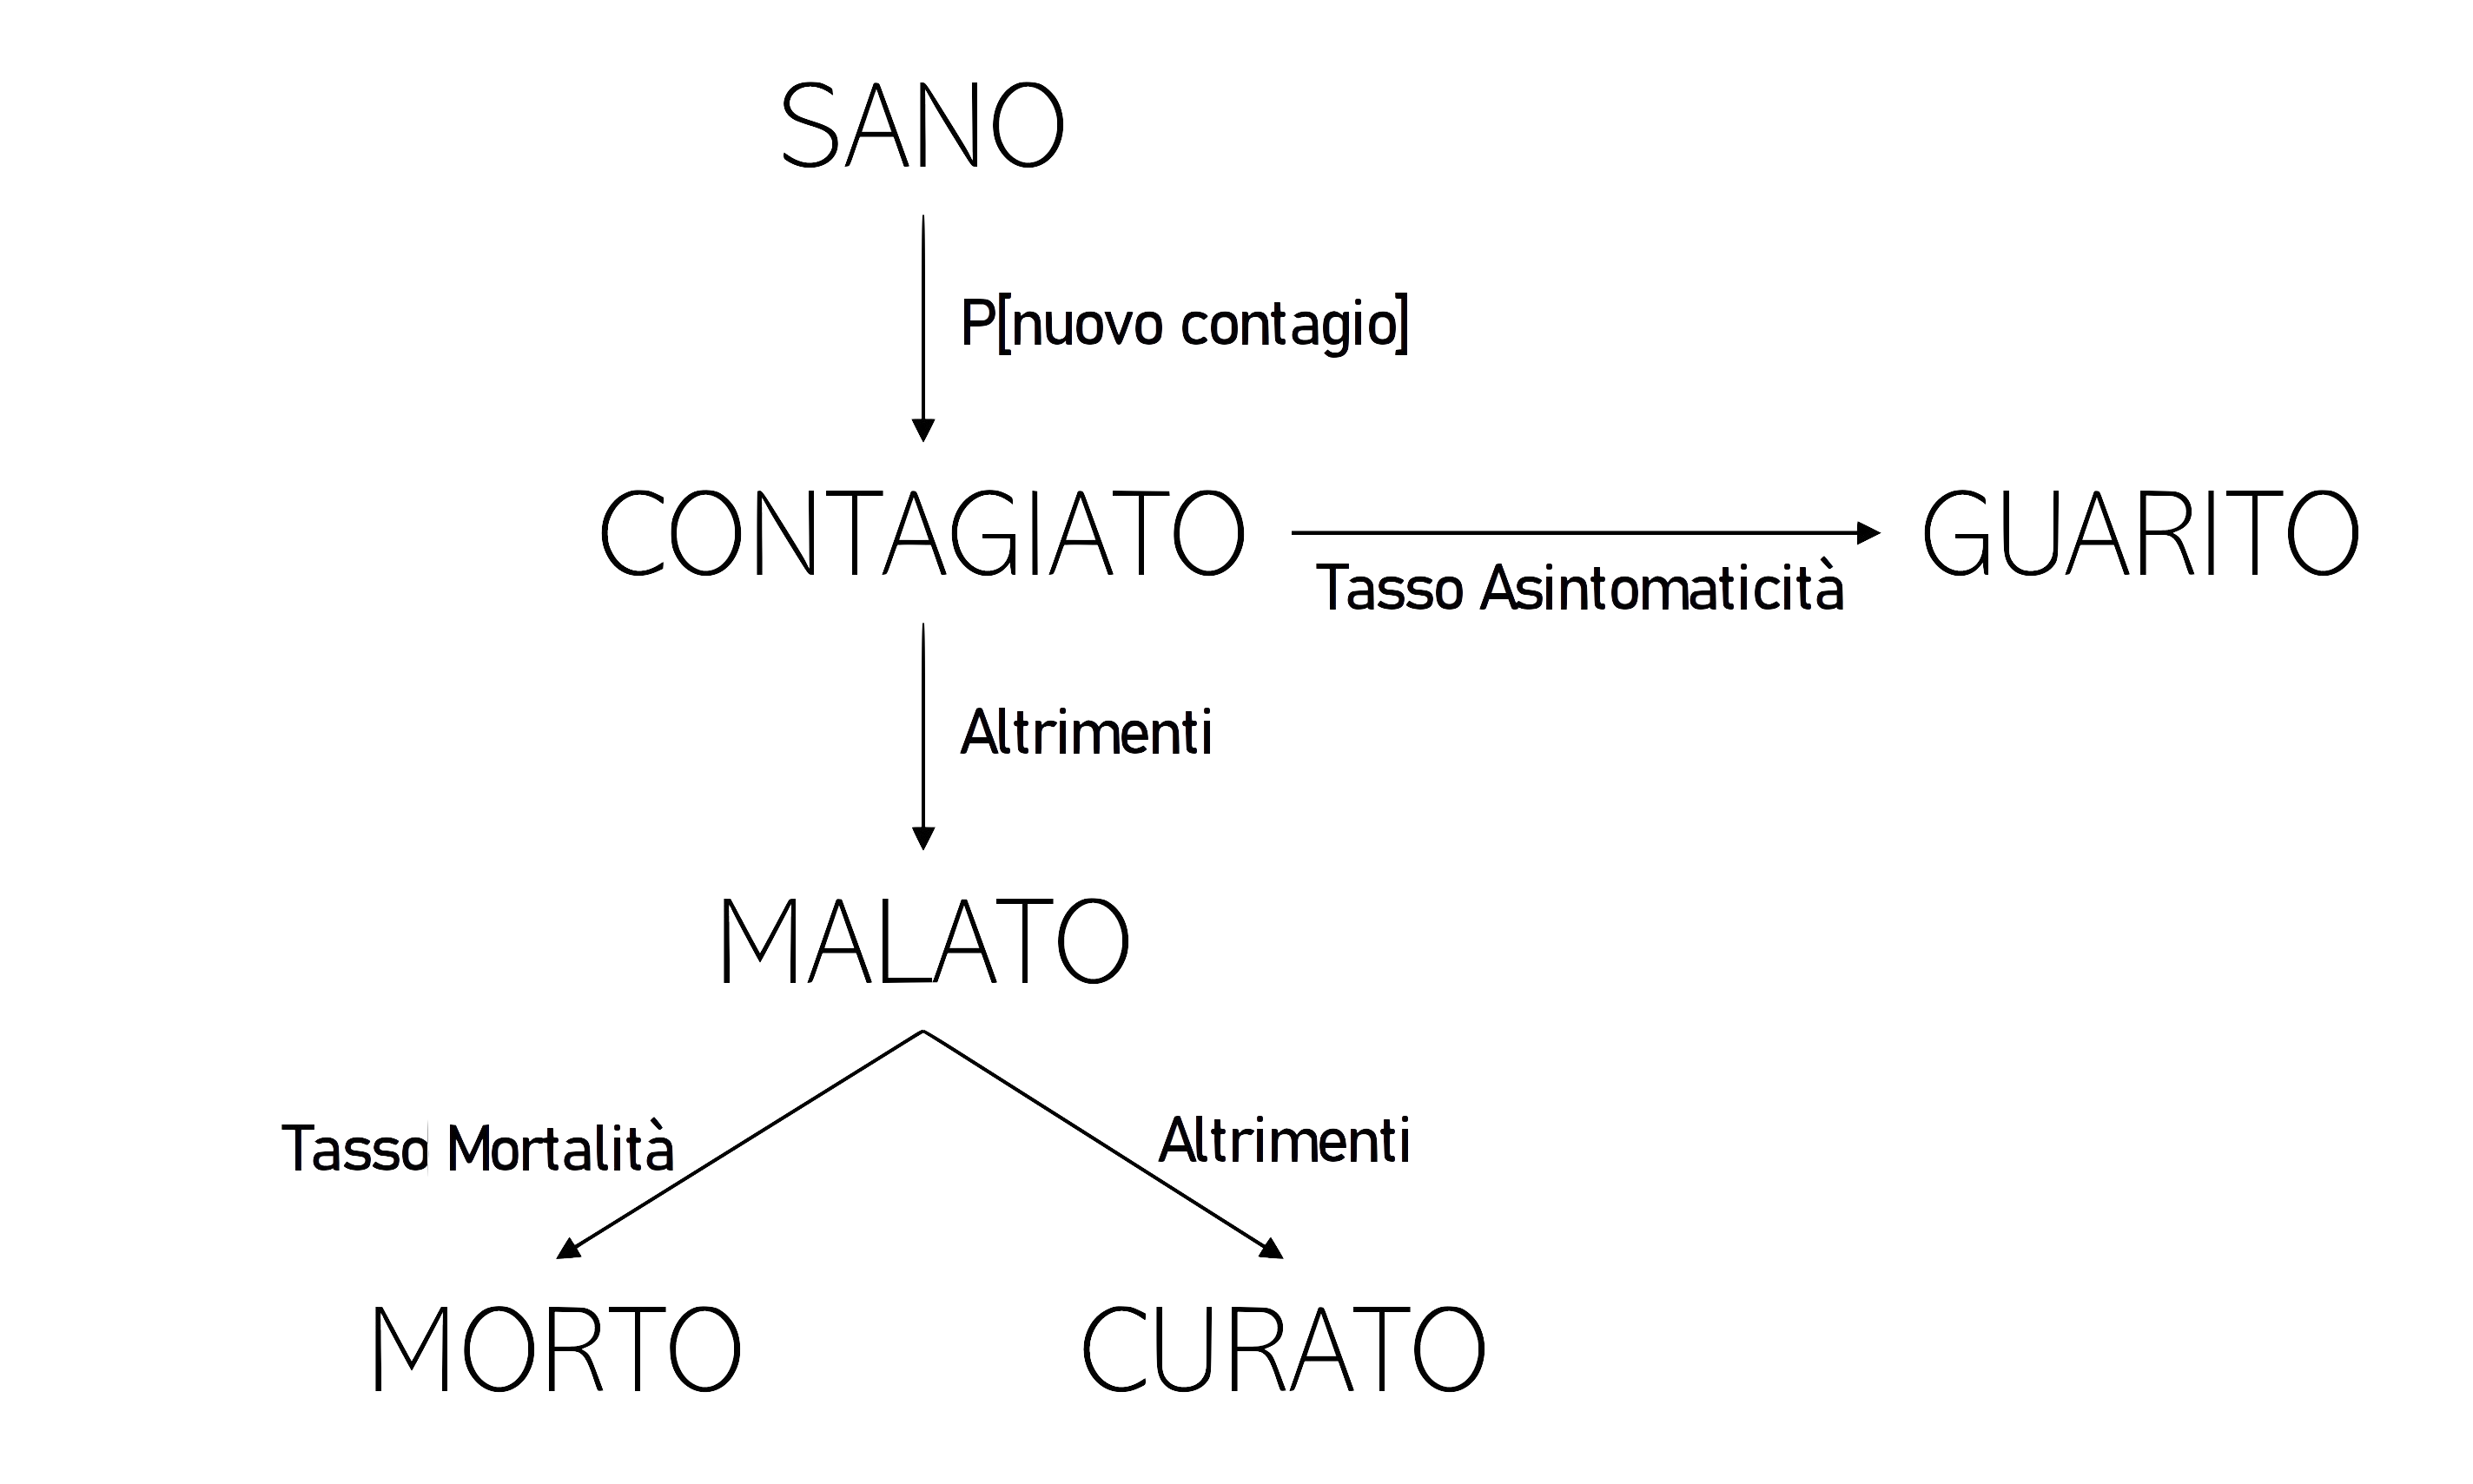
\includegraphics[width=1\textwidth]{IMG/FlowchartStatus.png}
		 	\caption[Cambio di stato]{}
		 	\label{fig:stati}
		 \end{figure}

	\subsection{AgeGroup}
		Per meglio rappresentare la realtà, la popolazione è divisa in tre macro classi di età:

		\begin{itemize}
			\item \textbf{SCUOLA:} fascia di età < 21 anni.
			\item \textbf{LAVORO:} fascia di età [21-65] anni.
			\item \textbf{PENSIONE:} fascia di età > 65 anni.
		\end{itemize}
	Per ognuna di queste classi sono impostabili diversi parametri che permettono un'elevata personalizzazione della simulazione.
	
	\subsection{HandlingType}
	Tipi di contromisure che possono essere prese, ognuna di esse ha un diverso impatto sull'evolversi del contagio e sono ordinate dalla più leggera alla più stringente:
	
	\begin{itemize}
		\item \textbf{NO\_ACT:} stato iniziale, quando nessuna misura di contenimento è stata presa.
		\item \textbf{REDUCED:} vengono inserite le contromisure base: come mascherine, distanziamento e attenzione generalizzata.
		\item \textbf{NO\_SCHOOL:} prime limitazioni alle libertà personali, chiusura delle scuole e dei luoghi più a rischio.
		\item \textbf{LOCKDOWN:} misura di massima gravità, il rischio di contagio è significativamente ridotto, ma ad un costo estremamente elevato.
	\end{itemize}
	Queste misure non vanno confuse con il concetto di chiusura: quest'ultima è la possibilità, garantita dal programma, di mettere in isolamento un ente, impedendo quindi al virus di uscire da esso.
	Tra queste due opzioni non c'è alcuna sovrapposizione e possono essere gestite in maniera totalmente indipendente l'una dall'altra: il fatto che un ente sia chiuso, infatti, non modifica in alcun modo la diffusione del virus all'interno dello stesso.

\newpage
% DESCRIZIONE

\section{Descrizione}
	
	Nei paragrafi che seguono, verranno analizzati da un punto di vista qualitativo alcuni aspetti dell'applicazione, ponendo particolare attenzione ai punti di forza, a quelli di debolezza e ai risultati auspicati che caratterizzano questo programma.
	
	\subsection{Contesto}
		Poiché ritengo il contesto essere chiaro a chiunque abbia passato gli ultimi 10 mesi su questo pianeta, non mi dilungherò troppo a lungo su questo punto.\\
		Voglio solo riportare alcuni numeri relativi all'Italia, perché non cadano nell'oblio: più di 35k decessi confermati, oltre 250k casi accertati, 2 mesi di lockdown quasi totale in tutto il Paese.\footnote{Dati forniti dalla Protezione Civile: \url{http://www.salute.gov.it/portale/nuovocoronavirus/dettaglioContenutiNuovoCoronavirus.jsp?id=5351&area=nuovoCoronavirus&menu=vuoto}}
	
	\subsection{Obiettivo}
		Il simulatore si prefigge lo scopo di offrire delle istantanee riguardo la diffusione del virus, permettendo quindi di confrontare (a parametri di base immutati) gli snapshot ottenuti mettendo in pratica misure differenti.\\
		I modelli, che ho incontrato durante la fase di studio per la creazione di questo progetto, erano puramente matematici: sistemi di complesse equazioni differenziali sì capaci di prevedere l'andamento dell'epidemia, ma in modo estremamente limitato, generico e complesso.
		L'approccio che ho deciso di seguire è invece decisamente più potente: una simulazione che si aggiorna automaticamente, relativa ad ogni singolo ente del Paese, che è quindi capace di regolarsi autonomamente e di interagire con i nodi  vicini; risultati impossibili con un approccio puramente matematico.
		Ogni iterazione modifica la ripartizione della popolazione tra i vari stati, permettendo di calcolare puntualmente tutte le evoluzioni e i cambiamenti.
		
		Questo programma offre un punto di vista unico della modellizzazione della pandemia, estremamente potente ma allo stesso tempo utilizzabile da chiunque: molto più simile ad un piacevole videogioco gestionale piuttosto che ad un freddo report di numeri.
		Il risultato ultimo di questo progetto è offrire una democratizzazione e un'interiorizzazione delle decisioni, dando la possibilità di apprezzare in prima persona i risultati che le nostre scelte avrebbero avuto, se fossimo stati noi nella "stanza dei bottoni".
		
	\subsection{Ipotesi semplificative}
		Nella stesura della logica del contagio sono state seguite alcune misure semplificative:
		
			\begin{itemize}
			\item La modellazione del virus è abbastanza semplice e si basa su una versione personalizzata e adattata della classica logica SIR (Suscettibili, Infetti, Rimossi).\footnote{\url{https://it.wikipedia.org/wiki/Modelli_matematici_in_epidemiologia}}\\
			Questo comporta che, dagli stati terminali GUARITO e CURATO, non si possa ritornare SANO; di conseguenza, una volta contratto il virus, non è possibile ammalarsi nuovamente. Non sono inoltre previsti altri possibili stati, come IMMUNE o VACCINATO.
			\item I parametri relativi alla popolazione, come ad esempio il tasso di mobilità o la suddivisione per fasce di età, sono considerati costanti su tutto il territorio nazionale. Questa approssimazione appiattisce inevitabilmente le specificità delle varie zone del paese, ma è sfortunatamente necessaria considerata l'estrema difficoltà nel reperimento di tali dati.
			\item Nella realtà i movimenti delle persone sono estremamente più complessi e imprevedibili; c'è inoltre la possibità di arrivi di persone contagiose provenienti dall'estero, che in questo modello non vengono considerate.
			\item Nella realtà non solo è possibile, ma è anche frequente, che si verifichino incontri di più persone contemporaneamente (esempio lampante sono i focolai), mentre questo modello considera soltanto incontri singoli tra 2 individui.
		\end{itemize}
		Molte di queste ipotesi possono essere allentate o fatte crollare, si veda la sezione \vref{sec:fut} per maggiori dettagli a riguardo.
		
	\subsection{Risultati}
		I risultati della simulazione sono visibili una volta raggiunta la condizione di terminazione, che non necessariamente coincide con la fine dell'epidemia: è infatti permesso interrompere la simulazione al raggiungimento di un determinato evento e di visualizzare i dati relativi a quel giorno.
		Le informazioni fornite per ogni singolo ente e livello di aggregazione sono:
		\begin{itemize}
			\item Il giorno in cui il virus è arrivato.
			\item La popolazione divisa per Status e AgeGroup sia in forma tabulare che come bar-graph.
			\item Il massimo valore di nuovi contagiati, malati, morti e il giorno in cui sono avvenuti.
			\item Alcuni line-chart per apprezzare l'evoluzione temporale degli stati più indicativi.
		\end{itemize}


\newpage
% DATABASE E GRAFO

\section{Struttura}

	\subsection{Database}
		
		Il database usato, allegato nella cartella \emph{db} del progetto\footnote{URI: \url{https://github.com/TdP-prove-finali/DebernardiLuca/tree/Mio/db}}, è una versione appositamente modificata e corretta di quello indicato nella sotto-sezione \vref{sub:db}.
		Esso si sviluppa su numerose tabelle, di cui alcune sono inutilizzate e altre potrebbero essere integrate direttamente a quelle a cui referenziano.
		Le tabelle principali sono quelle relative a Comuni, Province e Regioni che, seppur ognuna con proprie specificità, presentano una struttura simile.
		Una rappresentazione estremamente qualitativa dei dati disponibili per ogni ente è la seguente:
		\begin{itemize}
			\item \textbf{Nome e Id:} utili per identificare gli enti e usati come chiavi esterne.
			\item \textbf{Popolazione:} numero di abitanti dell'ente selezionato.
			\item \textbf{Superficie:} estensione in km$^{2}$ dell'ente.
			\item \textbf{Posizione:} per i comuni viene ricavata tramite i campi "lat" e "long"; mentre per le province e le regioni essa è ricavata come media delle posizioni di tutti i comuni che sono in essa presenti.
			\item \textbf{Superiori:} permettono di ricavare gli enti, di un livello di aggregazione superiore, che comprendono quello selezionato.\\
			Esempio: (Torino $\to$ TO, Piemonte).
		\end{itemize}

	\subsection{Grafi}
		Ebbene sì, il modello si serve non di uno, ma di ben tre grafi per svolgere la simulazione:
		\begin{itemize}
			\item \textbf{Regioni:} Il grafo essenziale per qualsiasi livello di aggregazione, esso permette di ottenere le adiacenze tra le varie regioni.
			Tutti gli archi sono ovviamente di tipo cross-regionale.
			Ogni regione è collegata con ogni altra. (20 N - 190 A)
			\item \textbf{Province:} grafo che gestisce lo spostamento tra province adiacenti.
			Viene creato solo se è richiesta una maggiore precisione rispetto al livello regionale. Gli archi possono essere non solo cross-provinciali ma anche cross-regionali. Le province sono collegate esclusivamente a quelle adiacenti (anche se di regioni diverse) e alla provincia del proprio capoluogo di regione. (107 N - 331 A)
			\item \textbf{Comuni:} grafo che offre la maggiore precisione, che viene creato soltanto se il livello di aggregazione scelto è quello comunale.
			Estremamente complesso, viene creato in tre passaggi:
			\begin{itemize}
				\item Vengono utilizzate le adiacenze delle province per cercare i comuni, appartenenti a province e regioni diverse, che sono confinanti tra loro.
				Questi archi sono solo di tipo cross-regionale o cross-provinciale.
				\item Si cerca, all'interno di ogni provincia, i comuni che rispettano il criterio di adiacenza. Questi archi sono solo di tipo cross-comunale.
				\item Si collega il capoluogo della provincia ad ogni altro comune della stessa. Anche questi archi possono essere solo cross-comunali.
			\end{itemize}
			Se non si seguissero questi 3 passaggi, ma si provasse a verificare l'adiacenza su tutte le 64 milioni di possibilità (32M di combinazioni), si otterrebbe un risultato perfettamente analogo, ma in un tempo decisamente più elevato. (7954 N - 39800 A)
		\end{itemize}
		Abbiamo parlato finora di adiacenze, ma poiché queste non sono indicate nel db, come sono state calcolate?
		Basare questo importantissimo criterio su un valore costante (es 10km) era un'approssimazione eccessiva, si sarebbero perse molte adiacenze in alcuni luoghi (grossi comuni adiacenti) e allo stesso tempo se ne sarebbero create troppe in altri (nuvole di comuni di piccolissime dimensioni); non era affidabile.
		Allora ho pensato di pesare la distanza sulla base della popolazione dei due comuni, ma anche qui non sempre le cose funzionano, ecco un esempio:
		\begin{itemize}
			\item Torino	\hfill 870.000 ab. \hspace{3cm} 130km$^{2}$
			\item Ceresole Reale (TO)	\hfill 167 ab. \hspace{3cm} 100km$^{2}$
		\end{itemize}
		L'unica soluzione ragionevole è quindi usare direttamente la dimensione dell'ente, la via più rapida è ricavare il raggio di questo a partire dalla superfice (considerata approssimabile ad un cerchio). Abbiamo quindi:
		\begin{equation}
			S = \pi r^{2} 	\quad \Rightarrow \quad r = \sqrt{\frac{S}{\pi}}
		\end{equation}
		Per ogni ente, se aggiungiamo questa informazione alla conoscenza del suo centro (fornito nel caso dei comuni; ricavato, come media della nuvola di comuni che le compongono, per province e regioni), possiamo creare la condizione di adiacenza come:
		\begin{equation}
		%\text{sono adiacenti se }
		d (A, B) \le k(r_{A}+r_{B})  
		\end{equation}
		dove $k$ è un coefficiente dovuto alla forma irregolare degli enti. Dopo verifiche sperimentali è stato posto $k = 1.5$.\\
		Se la distanza tra i due enti non è superiore alla somma aggiustata dei due raggi, allora la condizione di adiacenza è verificata.

\newpage
% LOGICA

\section{Logica}
	\label{sec:log}
	Siamo giunti alla parte più importante di tutto il codice, l'algoritmo vero e proprio;
	esso si compone di due parti e viene ripetuto ad ogni iterazione (che corrisponde ad ogni nuovo giorno della simulazione).
	
	\subsection{Interazioni}
		La prima riguarda le interazioni tra gli enti del nostro grafo (il cui livello di aggregazione corrisponde all'AggregationType scelto per la simulazione).\\
		Durante questo processo, si viene a creare una suddivisione della popolazione che è differente da quella effettiva: infatti il numero di individui contagiosi non è più soltanto quello dell'ente specifico, ma è calcolato anche sulla base di quello dei nodi a lui direttamente collegati.\\
		Più precisamente, un ente distribuisce ai nodi adiacenti una popolazione di contagiosi pari alla porzione della propria che si muove fuori dal comune.
		Ogni aggregazione ha un tasso di movimento diverso, modificabile a piacere nell'applicazione.
		Questa porzione di popolazione è distribuita a ciascun nodo adiacente all'ente selezionato, sulla base del numero di residenti di quel nodo rispetto alla popolazione totale dei nodi adiacenti, come mostrato dalla figura \vref{fig:dist}.
		\begin{figure}[H]
			\centering
			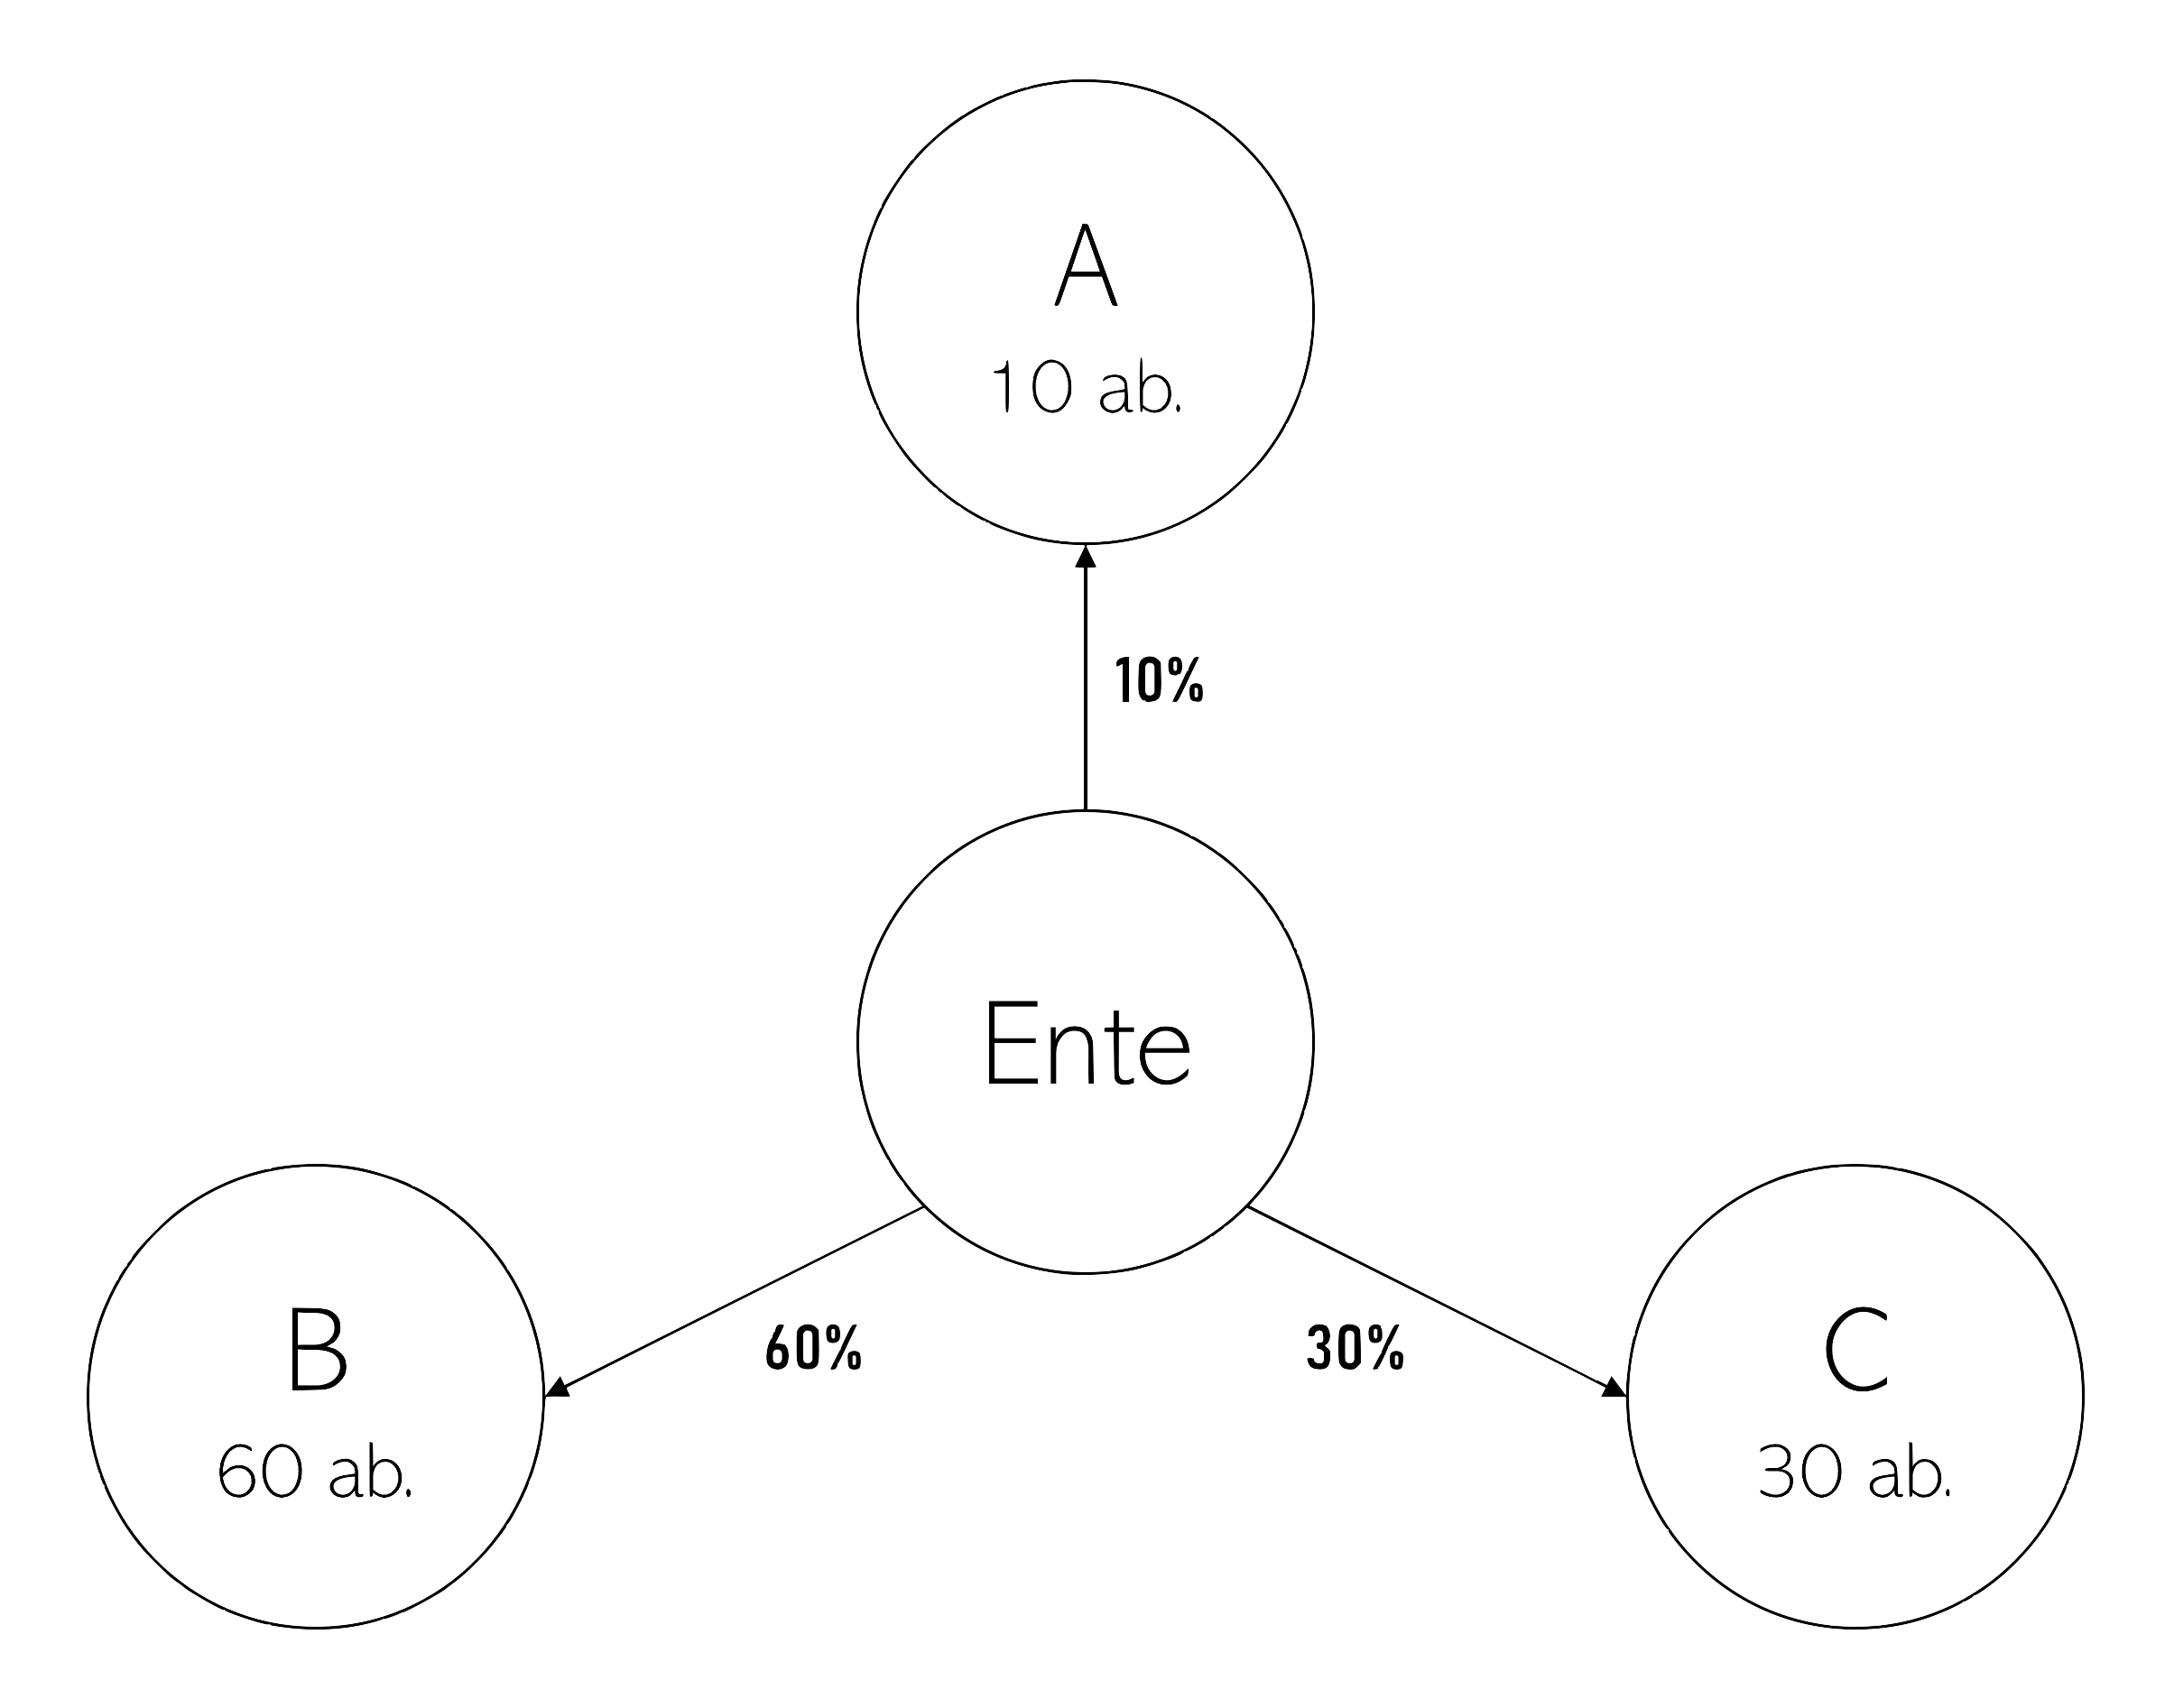
\includegraphics[width=0.75\textwidth]{IMG/diffusione.png}
			\caption[Ridistribuzione della popolazione]{Schema che esemplifica la ridistribuzione (in percentuale) della popolazione mobile di un ente nei suoi nodi adiacenti.}
			\label{fig:dist}
		\end{figure}
		Se l'AggregationType è di tipo comunale, oltre alla relazione tra i comuni, viene attuata anche quella tra le province (la popolazione viene attribuita ai capoluoghi di provincia, sulla base delle province adiacenti) e tra le regioni (su tutte le altre regioni). Discorso analogo, ma più ristretto, se l'aggregazione è provinciale.
		In caso un ente sia chiuso, gli archi partenti da questo non vengono considerati.
		Più specificatamente, se il Piemonte venisse chiuso, nessun arco (a qualunque livello di aggregazione), che esce dai confini regionali, entrerebbe nel calcolo; ma ciò non modificherebbe il movimento all'interno dell'ente. Se si volesse limitare al massimo lo spostamento al suo interno, sarebbe necessario chiudere anche tutti i comuni e le province che lo compongono.
		
		
		La complessità di questa parte deriva dalla necessità di controllare tutte le adiacenze, quindi il numero di archi: O(A).
		
	\subsection{Aggiornamento}
		In questa seconda parte avviene, per ogni ente, l'aggiornamento delle sue popolazioni effettive.
		Ogni passaggio di stato segue un ragionamento diverso:
		\begin{itemize}
			\item \textbf{SANO $\to$ CONTAGIOSO:} Passaggio focale della simulazione, usa le popolazioni fittizie create in precedenza per cercare la probabilità che, da un incontro, si sviluppi un contagio.
			Prima di tutto bisogna capire il concetto di contatto a rischio:
			Definiamo S, C, F come numero rispettivamente delle persone SANE, CONTAGIOSE e FREE.
			Usiamo il pedice "$_{m}$" per mettere in evidenza che non si tratta delle popolazioni effettive dell'ente, ma di quelle ricavate, nel punto precedente, tramite gli indici di mobilità.\\
			Il numero di contatti totali è:
			\begin{equation}
				N_{t} = \dfrac{F_{m} (F_{m}-1)}{2}
			\end{equation}
			Ovvero tutte le possibili combinazioni di incontri (utilizzando come semplificazione che questi incontri possano avvenire \textbf{solo tra 2 persone}).
			Se ho un mondo di 4 persone, sono quindi possibili 6 contatti diversi.\\
			%, provare per credere.\\
			Il numero di contatti a rischio è invece:
			\begin{equation}
				N_{r} = S_{m} C_{m}
			\end{equation}
			Chiaramente se nel mio mondo ho 3 persone sane e una malata, gli unici contatti che possono trasmettere il contagio sono quelli tra uno dei sani e il malato, quindi $3*1 = 3$ contatti a rischio.\\
			La probabilità che si verifichi un contatto a rischio è:
			\begin{equation}
				P[r] = \dfrac{N_{r}}{N_{t}}
			\end{equation}
			Nel nostro mondo quindi solo il 50\% dei contatti potrebbe portare ad un contagio.\\
			Posta $B_{0}$ la probabilità che, in condizioni standard, da un contatto a rischio derivi un nuovo contagio, la probabilità che un individuo venga contagiato se in quel giorno ha incontrato una persona è:
			\begin{equation}
				P[c] = k_{adj} B_{0} P[r] = k_{adj} B_{0} \dfrac{2 S_{m} C_{m}}{F_{m}(F_{m}-1)}
			\end{equation}
			dove $k_{adj}$ è un correttore che tiene in considerazione la densità dell'ente rispetto alla densità media del paese e il livello di contromisure adottato ($B_{1} = k_{adj} B_{0}$).\\
			Infine, Il valore atteso dei nuovi contagi è dato dalla probabilità che una persona diventi contagiata, moltiplicata per il numero di persone che possono creare contatti, ovvero:
			\begin{equation}
				E[C_{new}] = P[c] F_{m} = k_{adj} B_{0} \dfrac{2 S_{m} C_{m}}{F_{m}-1}
			\end{equation}
			\item La logica che regola gli altri 4 possibili passaggi di stato è molto più semplice: prima di tutto bisogna capire il numero di persone che effettuerà questo cambio.
			Due dei parametri (modificabili) del virus sono il tempo medio da CONTAGIOSO e quello da MALATO.
			Quindi, il tasso con cui una persona passa da uno stato all'altro è:
			\begin{equation}
				r_{c} = \dfrac{1}{t_{c}}
			\end{equation}
			che corrisponde alla probabilità che un individuo cambi di stato.\\
			Se ciò accade la persona viene immediatamente assegnata, a seconda delle probabilità in gioco, ad uno dei due stati successivi.
		\end{itemize}
		C'è ancora un'ultima precisazione da fare, che riguarda il SimulationType scelto:
		\begin{itemize}
			\item \textbf{SEMI\_DETERMINISTICO:} Modalità leggera di simulazione che si basa sul valore atteso. Se mi aspetto di avere 5.8 nuovi contagi, c'è una probabilità dell'80\% che il valore effettivo sia 6 e del 20\% che sia 5.
			\item \textbf{STOCASTICO:} Modalità estremamente più pesante che, per ogni singolo individuo della popolazione, valuta se il cambio avvenga o meno.
			Se ho una popolazione di 100 individui e una probabilità del 10\%, potrei ottenere che tutti e 100 cambino di stato ($P = 0.1^{100}$) o che nessuno lo faccia ($P = 0.9^{100}$) e ovviamente qualsiasi altra delle possibilità intermedie; mentre con la modalità precedente otterrei sempre il valore atteso (fisso) di 10.
			
			Il rovescio della medaglia è che in questo caso il collo di bottiglia non è più determinato, come vedremo a breve, dal numero di nodi; ma dalla popolazione (in stato non terminale) del mio sistema, quindi inizialmente $O(P_{t})$, dove $P_{t} = 60M$ nel caso italiano.
		\end{itemize}
		La complessità di questa seconda parte deriva dalla necessità di modificare tutti i nodi, quindi O(N).
	
		
\newpage
% COMPOSIZIONE
		
\section{Composizione}
	L'applicazione, scritta in linguaggio Java, è stata creata utilizzando la libreria JavaFX.
	Nella sua progettazione sono stati implementati i pattern di buona programmazione:
	\begin{itemize}
		\item \textbf{DAO:} \emph{(Data Access Object)}, che si preoccupa di gestire il DB.
		\item \textbf{MVC:} \emph{(Model View Controller)}, per allocare in maniera ottimale le funzioni alle classi.
	\end{itemize}
	Essa si compone di \emph{19 classi}, suddivise in \emph{4 packages}, per un totale di oltre \emph{5000 LOC} \emph{(Lines Of Code)}.
	
	\subsection{Classi}
		Nelle pagine seguenti verranno mostrati i diagrammi UML delle classi principali; una versione più completa del diagramma è disponibile alla URI: \url{https://github.com/TdP-prove-finali/DebernardiLuca/tree/Mio/Documents/IMG/UML}
	
	\subsubsection{Model}
		Questa è la classe per eccellenza, dove è contenuta tutta la logica applicativa del programma.\\
		Il diagramma UML degli attributi è disponibile nella figura  \vref{fig:UMLmodel1}.\\
		Il diagramma UML dei metodi è disponibile nella figura  \vref{fig:UMLmodel2}.
		
	\subsubsection{StatisticheEnte}
		Classe che gestisce la parte di codice relativa alle statistiche e che è attribuita ad ogni singolo ente.\\
		Il diagramma UML è disponibile nella figura  \vref{fig:UMLstats}.
	
	\subsubsection{Parametri}
		Sono le classi che gestiscono i parametri relativi a virus, mondo e simulazione.\\
		Il diagramma UML è disponibile nella figura  \vref{fig:UMLpar}.
		
		\begin{figure}[H]
			\centering
			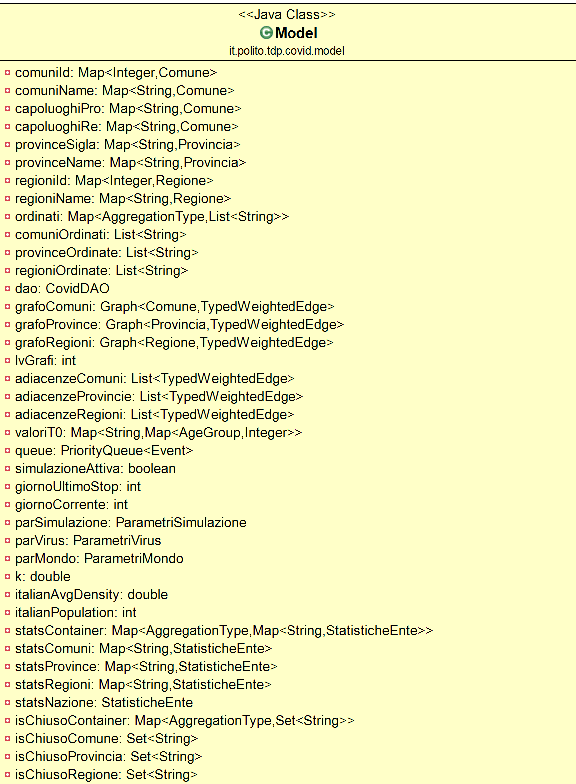
\includegraphics[width=\linewidth]{IMG/model_1.png}
			\caption[UML attributi modello]{Attributi della classe Model.}
			\label{fig:UMLmodel1}
		\end{figure}
		
		\begin{figure}[H]
			\centering
			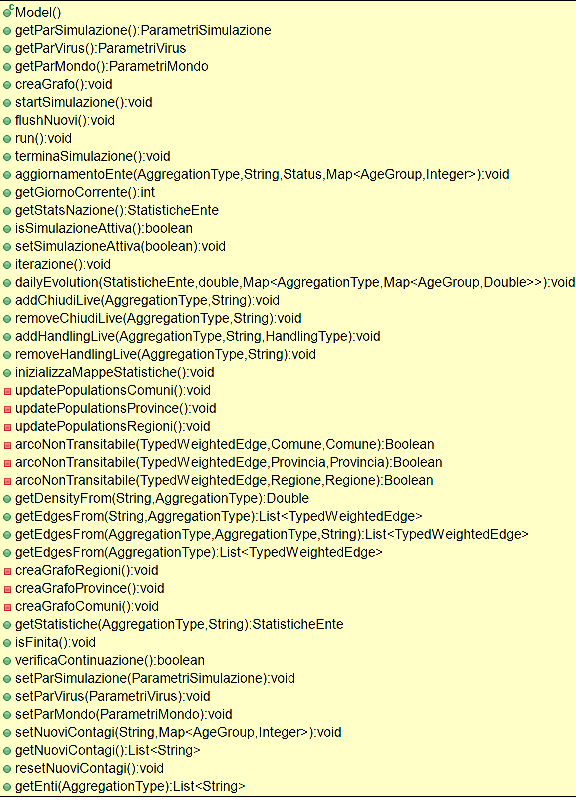
\includegraphics[width=\linewidth]{IMG/model_2.png}
			\caption[UML metodi modello]{Metodi della classe Model.}
			\label{fig:UMLmodel2}
		\end{figure}
	
		\begin{figure}[H]
			\centering
			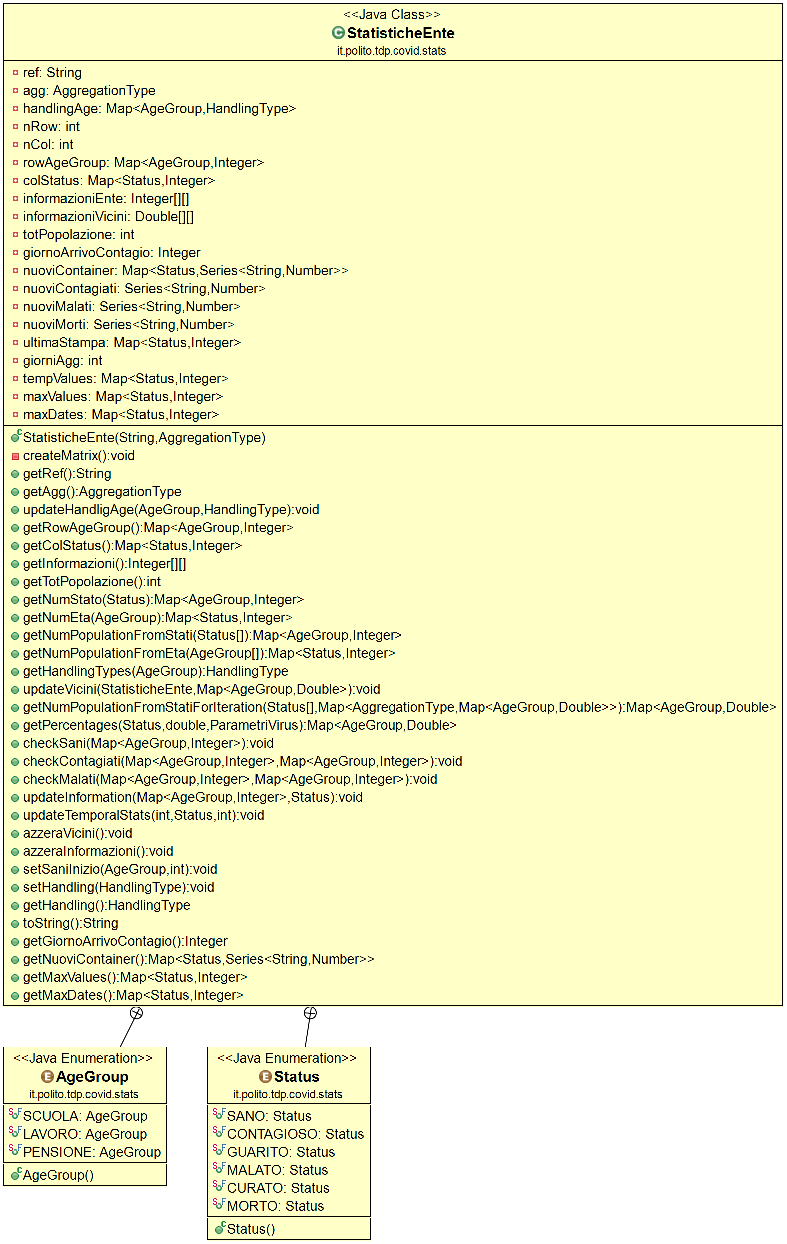
\includegraphics[width=\linewidth]{IMG/stats.png}
			\caption[UML statistiche]{Classe StatisicheEnte.}
			\label{fig:UMLstats}
		\end{figure}

		\begin{figure}[H]
			\centering
			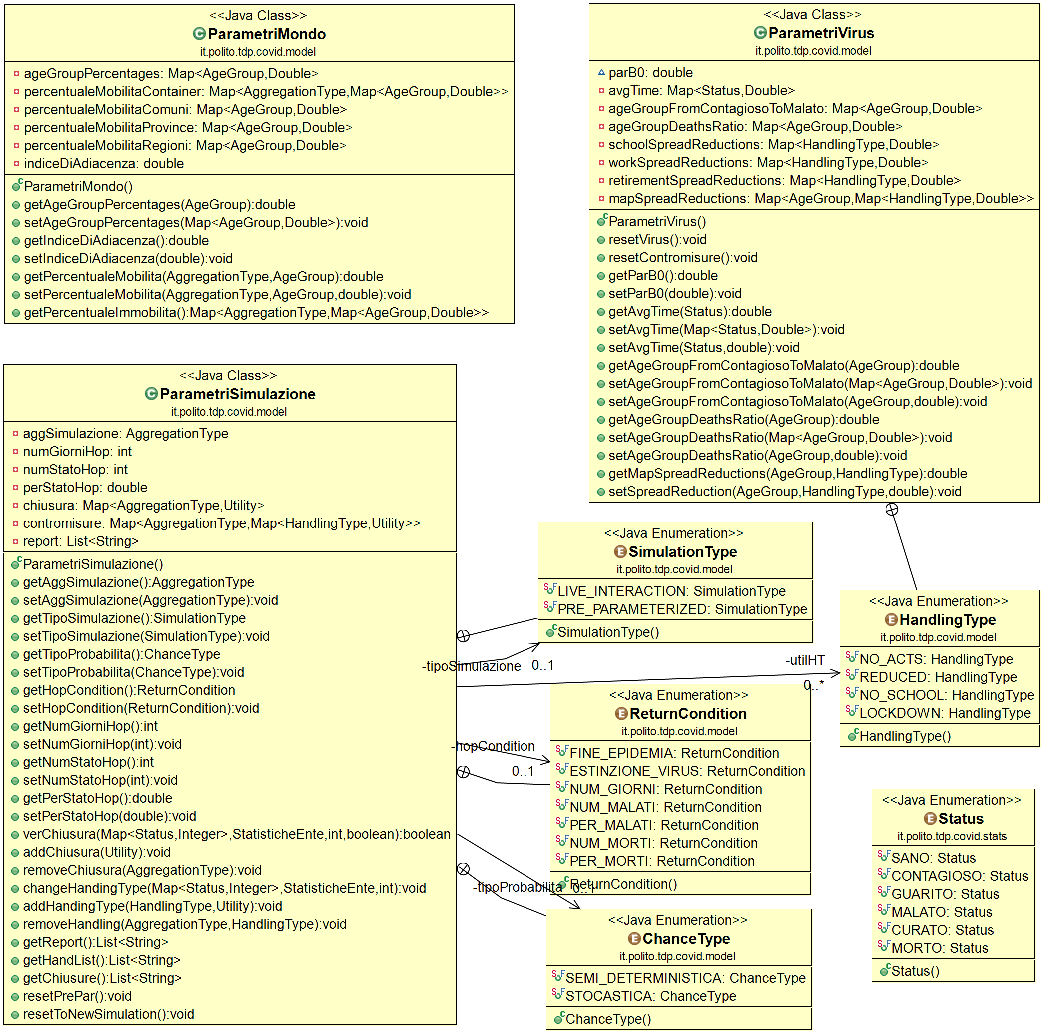
\includegraphics[width=\linewidth]{IMG/parametri.png}
			\caption[UML parametri]{Le tre classi che gestiscono i vari parametri.}
			\label{fig:UMLpar}
		\end{figure}

		
\newpage
% SCHERMATE

\section{Possibilità}
	Ora che abbiamo un'idea di massima di come l'applicazione funzioni, è arrivato finalmente il momento di scoprire quali sono le sue possibilità.		
	Innanzitutto, perché qualsiasi malattia possa partire, c'è bisogno di un "paziente 0".
	È quindi possibile scegliere, tramite un menù a tendina, uno o più enti da dove far partire il contagio.\\
	Se non si volesse identificare un punto preciso, è comunque possibile demandare all'applicazione la scelta casuale della località e/o del numero di infetti (quest'ultimo compreso nell'intervallo $[1-11]$ per ciascuna classe di età).
	
	Tutti i parametri usati dal programma sono modificabili dagli appositi Tab dell'interfaccia; in caso si voglia tornare ai valori preimpostati, è sufficiente premere il pulsante \emph{RESET}.
	Una volta impostati tutti i parametri, nel Tab \emph{Simulazione} è possibile scegliere la condizione di terminazione.
	Sono possibili due tipi di simulazione:
	\begin{description}
		\item[Pre-Parametrizzata:] Questa tipologia permette di scegliere a quali condizioni un ente vada isolato o una determinata contromisura debba attivarsi (facendo aumentare o diminuire il livello di gravità dell'HandlingType).
		Tali azioni posso essere eseguite in modo totalmente indipendente l'una dall'altra.
		Per fare ciò è sufficiente impostare (per ciascuno dei precedenti) il valore soglia\footnote{Può essere sia una percentuale della popolazione totale, sia un valore assoluto.} di malati o morti.
		La chiusura e la riapertura di un ente, così come il passaggio tra i diversi livelli di gravità delle contromisure, sono totalmente automatici e possono muoversi in entrambi i sensi.
		\item[Live:] Si ha la piena libertà, per qualsiasi ente, di obbligarne la chiusura o di modificarne il livello delle contromisure.\\
		Dato che queste modifiche possono essere attuate solo a simulazione in pausa, per poter agire in modo attivo è consigliabile impostare una condizione di terminazione diversa dalla fine dell'epidemia.
	\end{description}

	Nella pagina contenente i risultati, sono disponibili i valori finali, divisi per \emph{Status} e \emph{AgeGroup}, della popolazione dell'ente selezionato. In aggiunta, per ciascuno di essi, sono disponibili le informazioni circa il giorno in cui l'epidemia è arrivata e quello in cui sono stati raggiunti i picchi di nuovi contagiosi, malati e morti (e il valore di tale picco).\\
	Nei ultimi due Tab sono invece disponibili sia i grafici dell'evoluzione temporale dell'epidemia, sia un diagramma a barre per visualizzare in maniera più immediata i valori finali. Per coerenza i grafici in questi due Tab sono sempre legati all'ente scelto nel Tab \emph{Risultati}.

	Se è stata scelta una condizione di terminazione diversa da \emph{FINE\_EPIDEMIA}, è possibile continuare la simulazione aggiornando, se necessario, la condizione e premendo su \emph{AVVIA SIMULAZIONE}.\\
	Se si vuole invece terminare la simulazione corrente (magari per iniziarne una nuova), è sufficiente premere il bottone \emph{TERMINA SIMULAZIONE}.
	
	
\newpage
% SCHERMATE

\section{Schermate}
	Nelle immagini successive è mostrato un semplice esempio di simulazione:
	\begin{itemize}
		\item Livello aggregazione: \hfill PROVINCIA \hspace{0.5cm} $\text{}$
		\item Parametri Virus: \hfill Standard \hspace{0.5cm} $\text{}$
		\item Parametri Contromisure: \hfill Standard \hspace{0.5cm} $\text{}$
		\item Parametri Mondo: \hfill Standard \hspace{0.5cm} $\text{}$
		\item Parametri Simulazione: \hfill Standard \hspace{0.5cm} $\text{}$
		\item Contromisure attive: \hfill Nessuna \hspace{0.5cm} $\text{}$
		\item Risultati: \hfill Italia \hspace{0.5cm} $\text{}$
	\end{itemize}
	
	
\begin{figure}[H]
	\centering
	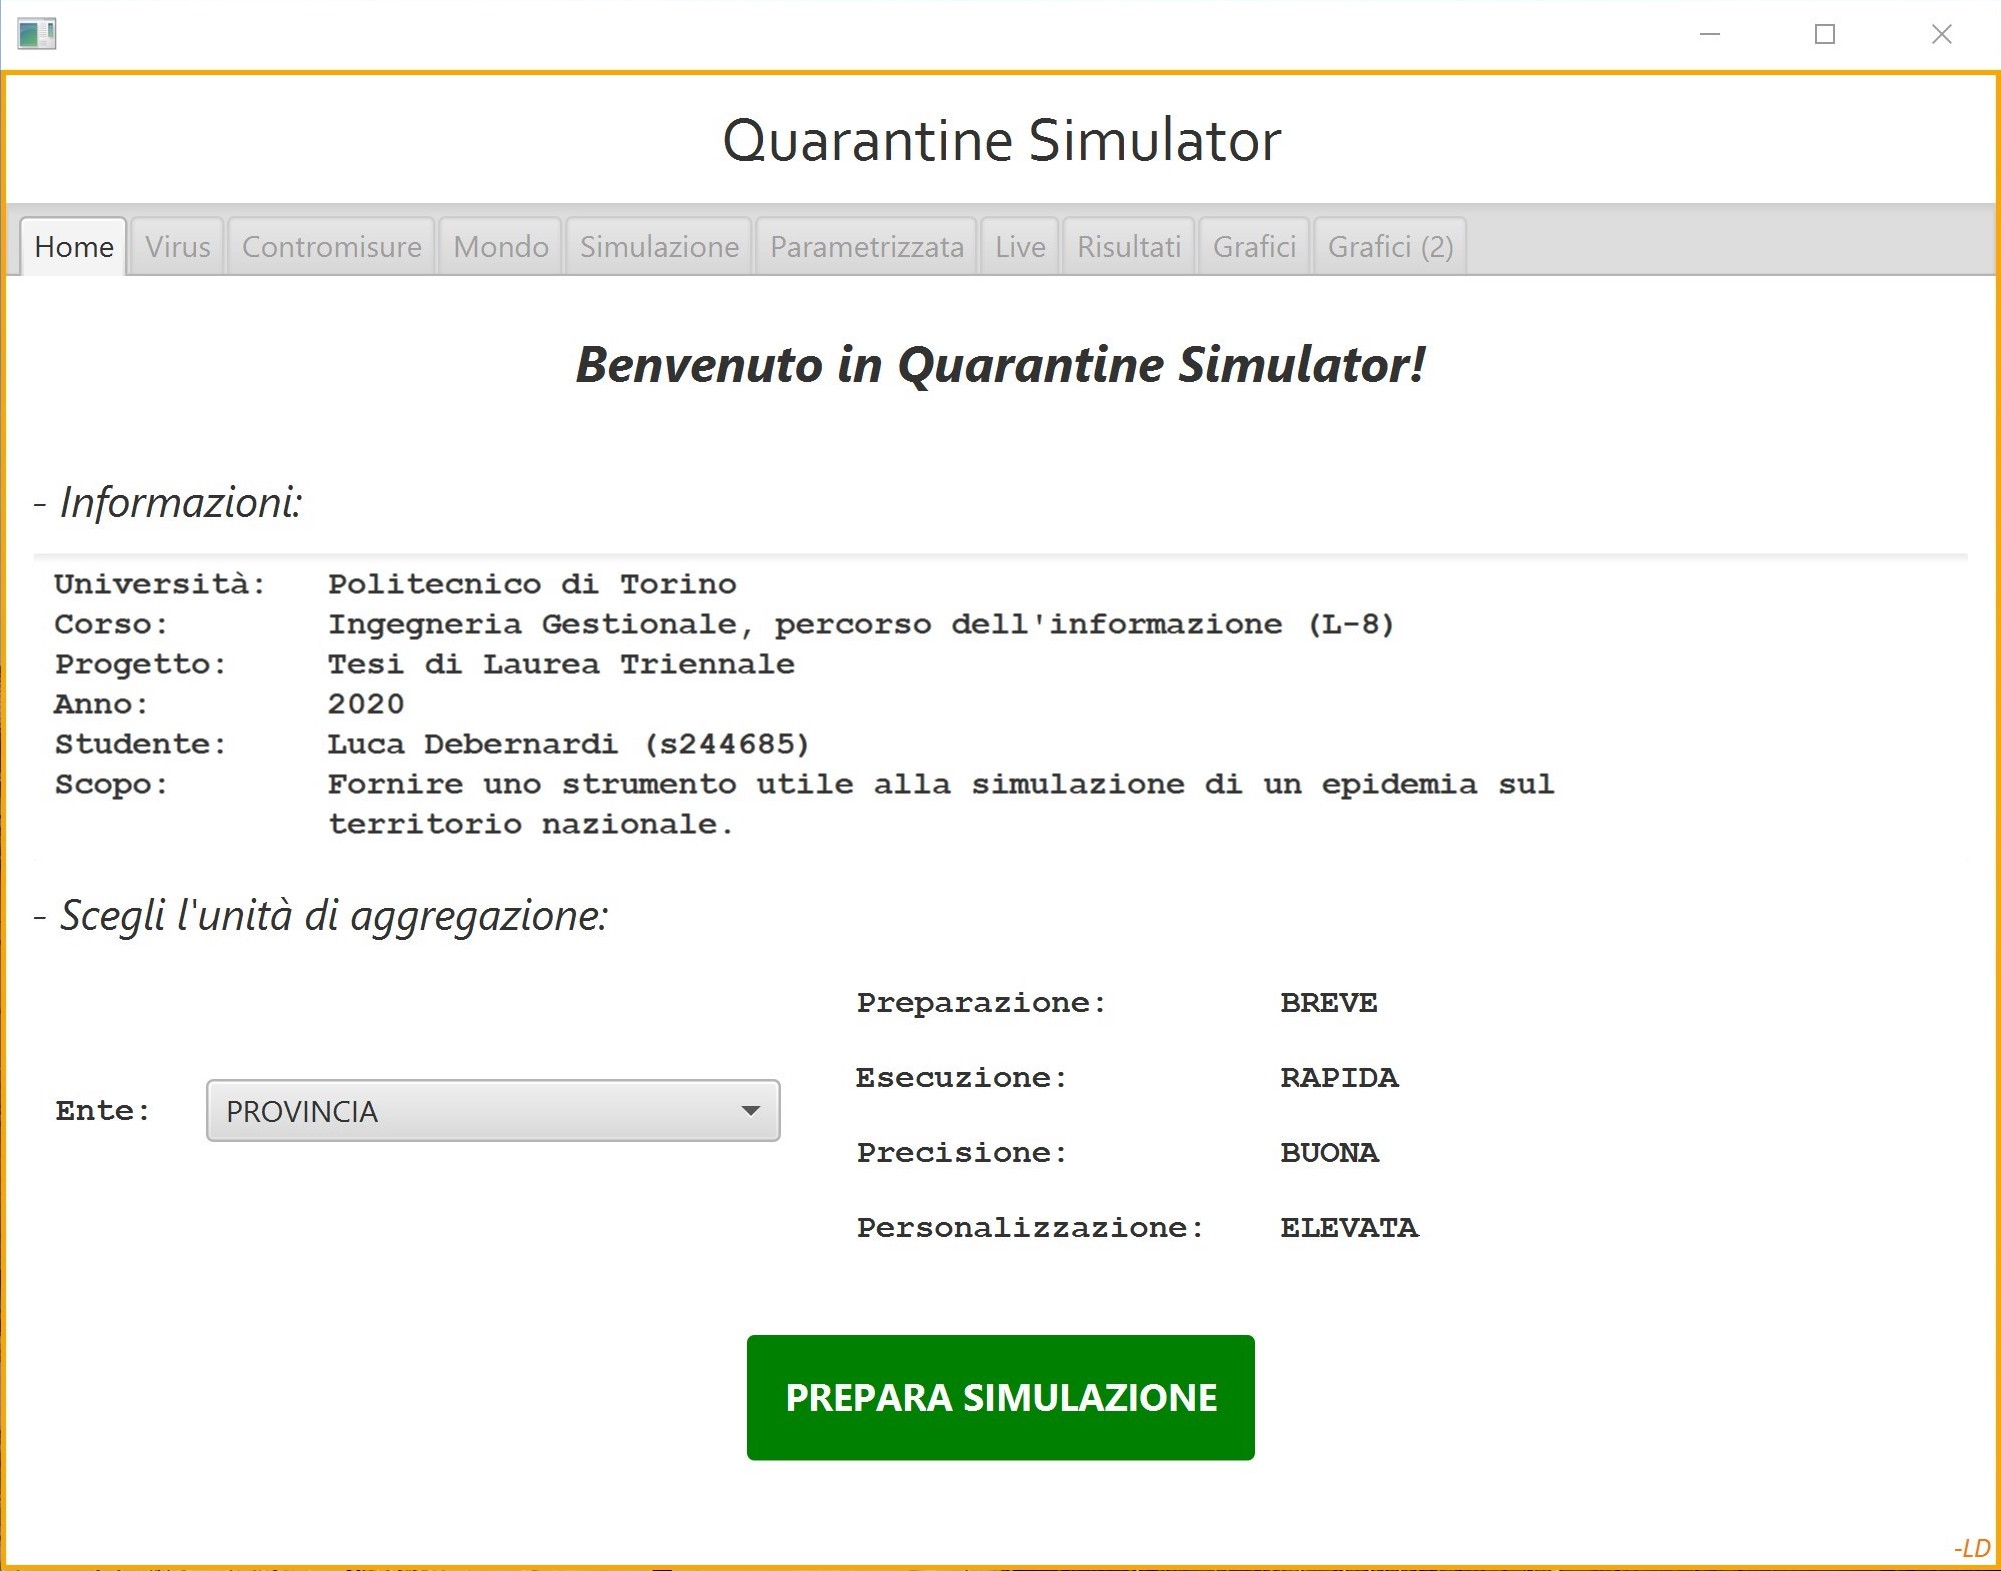
\includegraphics[height=0.4\textheight]{IMG/1.jpg}
	\caption[App: Tab Home]{Prima pagina mostrata all'apertura del programma: permette la scelta del livello di aggregazione.}
	\label{fig:screen1}
\end{figure}

\begin{figure}[H]
	\centering
	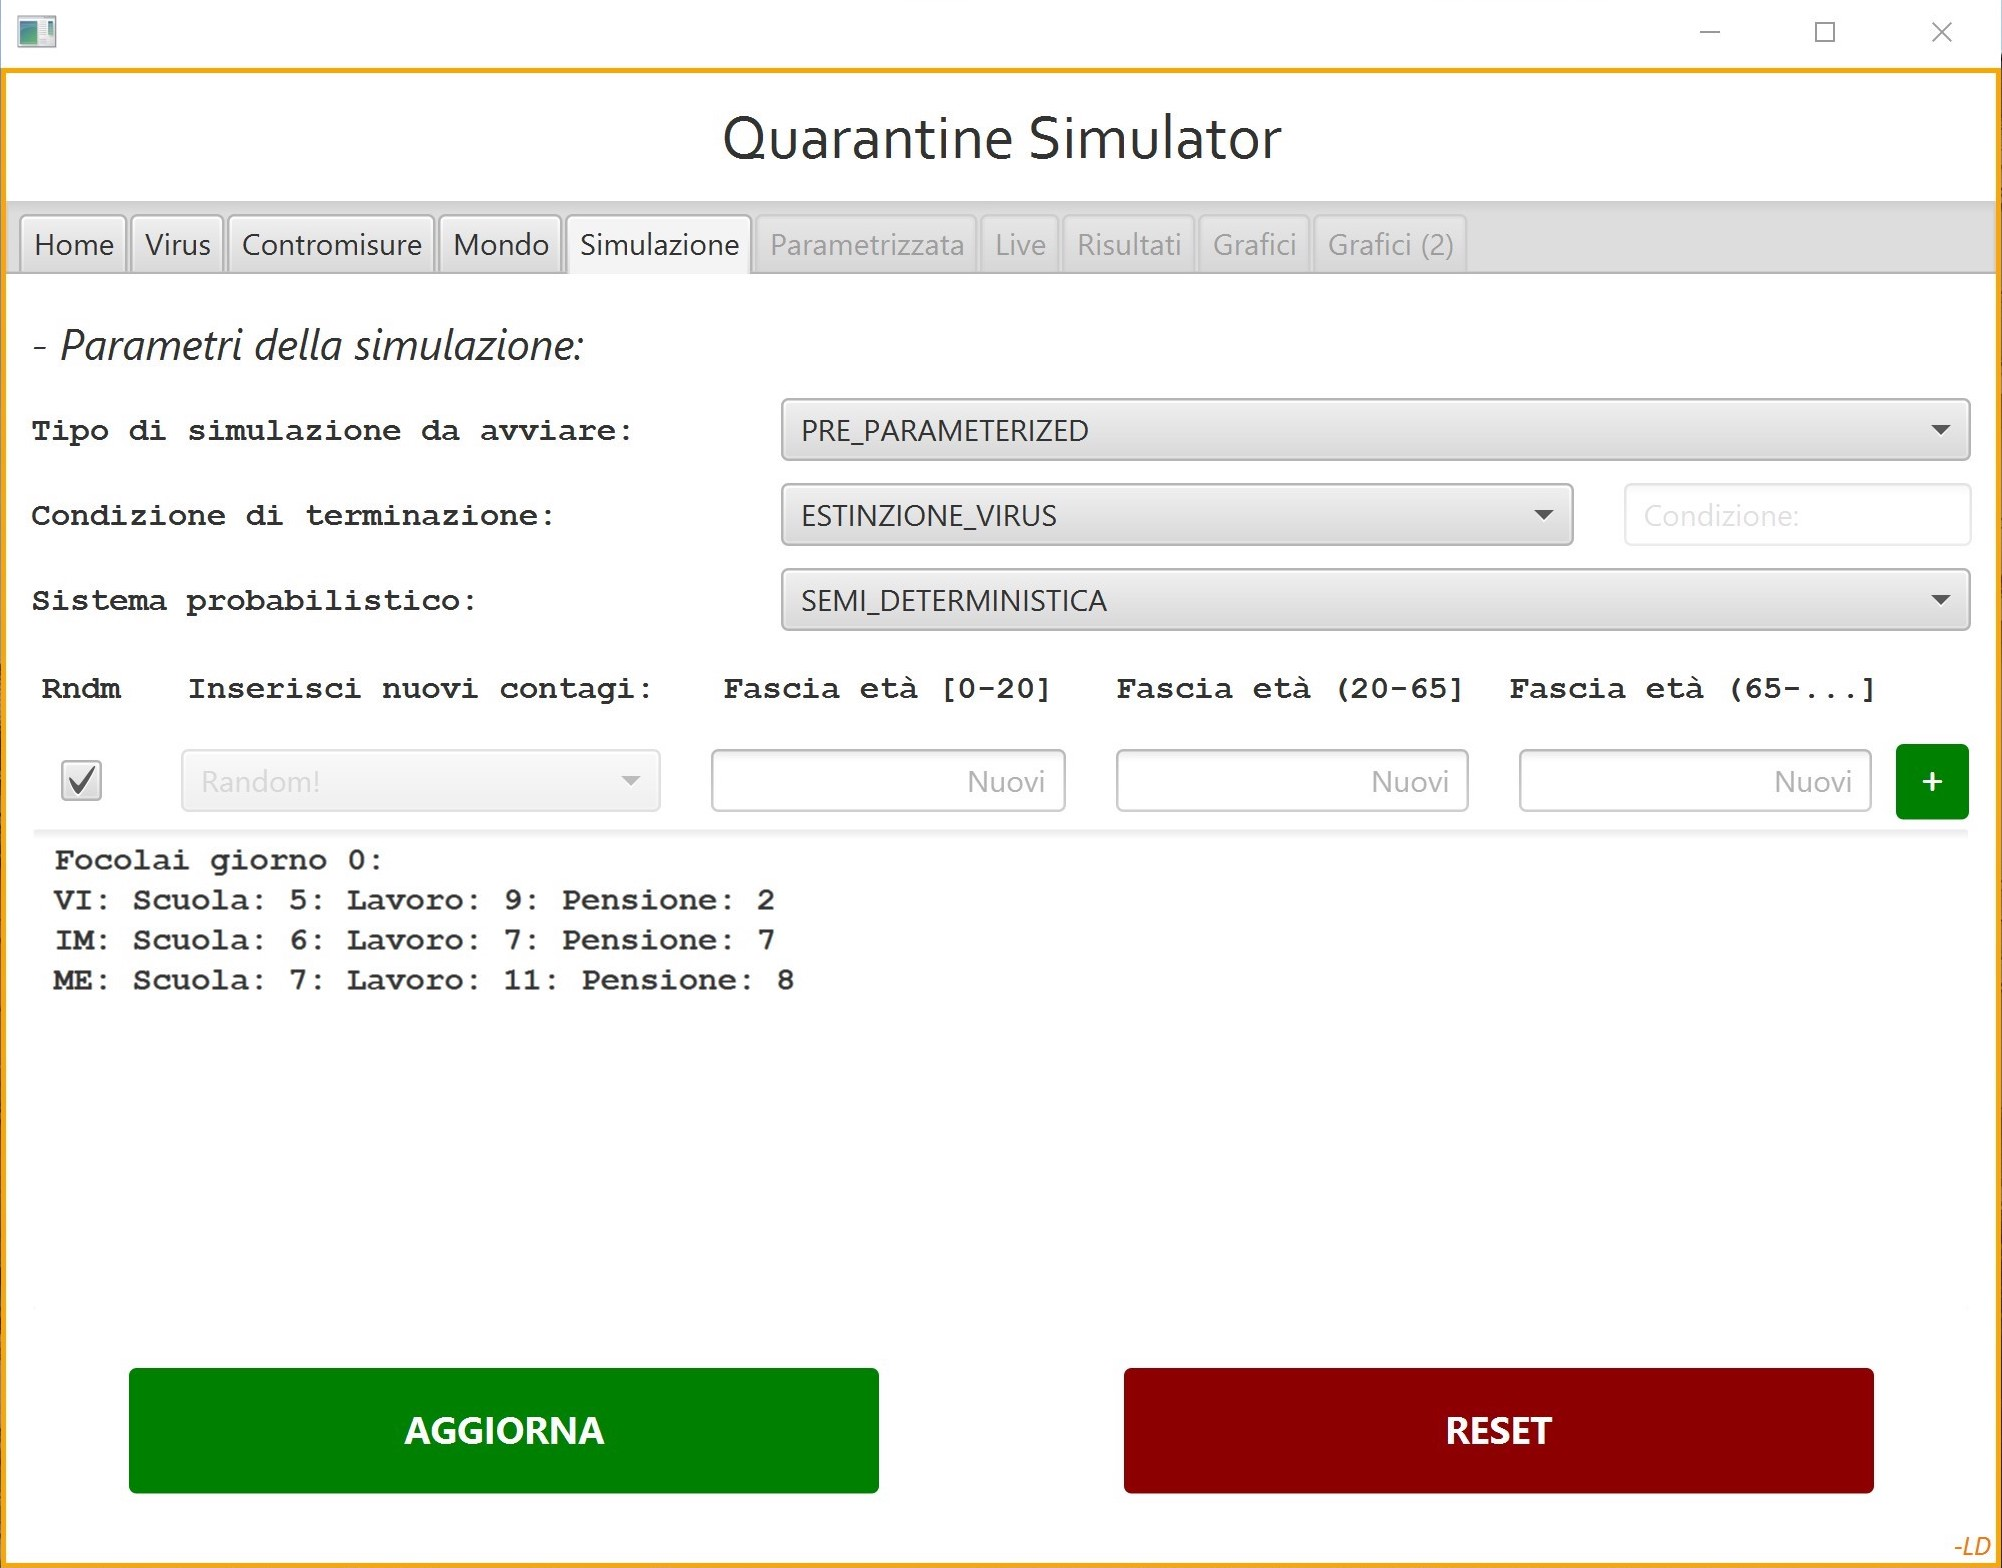
\includegraphics[height=0.4\textheight]{IMG/2.jpg}
	\caption[App: Tab Simulazione]{Tab in cui è possibile modificare i parametri di simulazione. In questo caso il contagio è iniziato dalle province di Vicenza, Imola e Messina.}
	\label{fig:screen2}
\end{figure}

\begin{figure}[H]
	\centering
	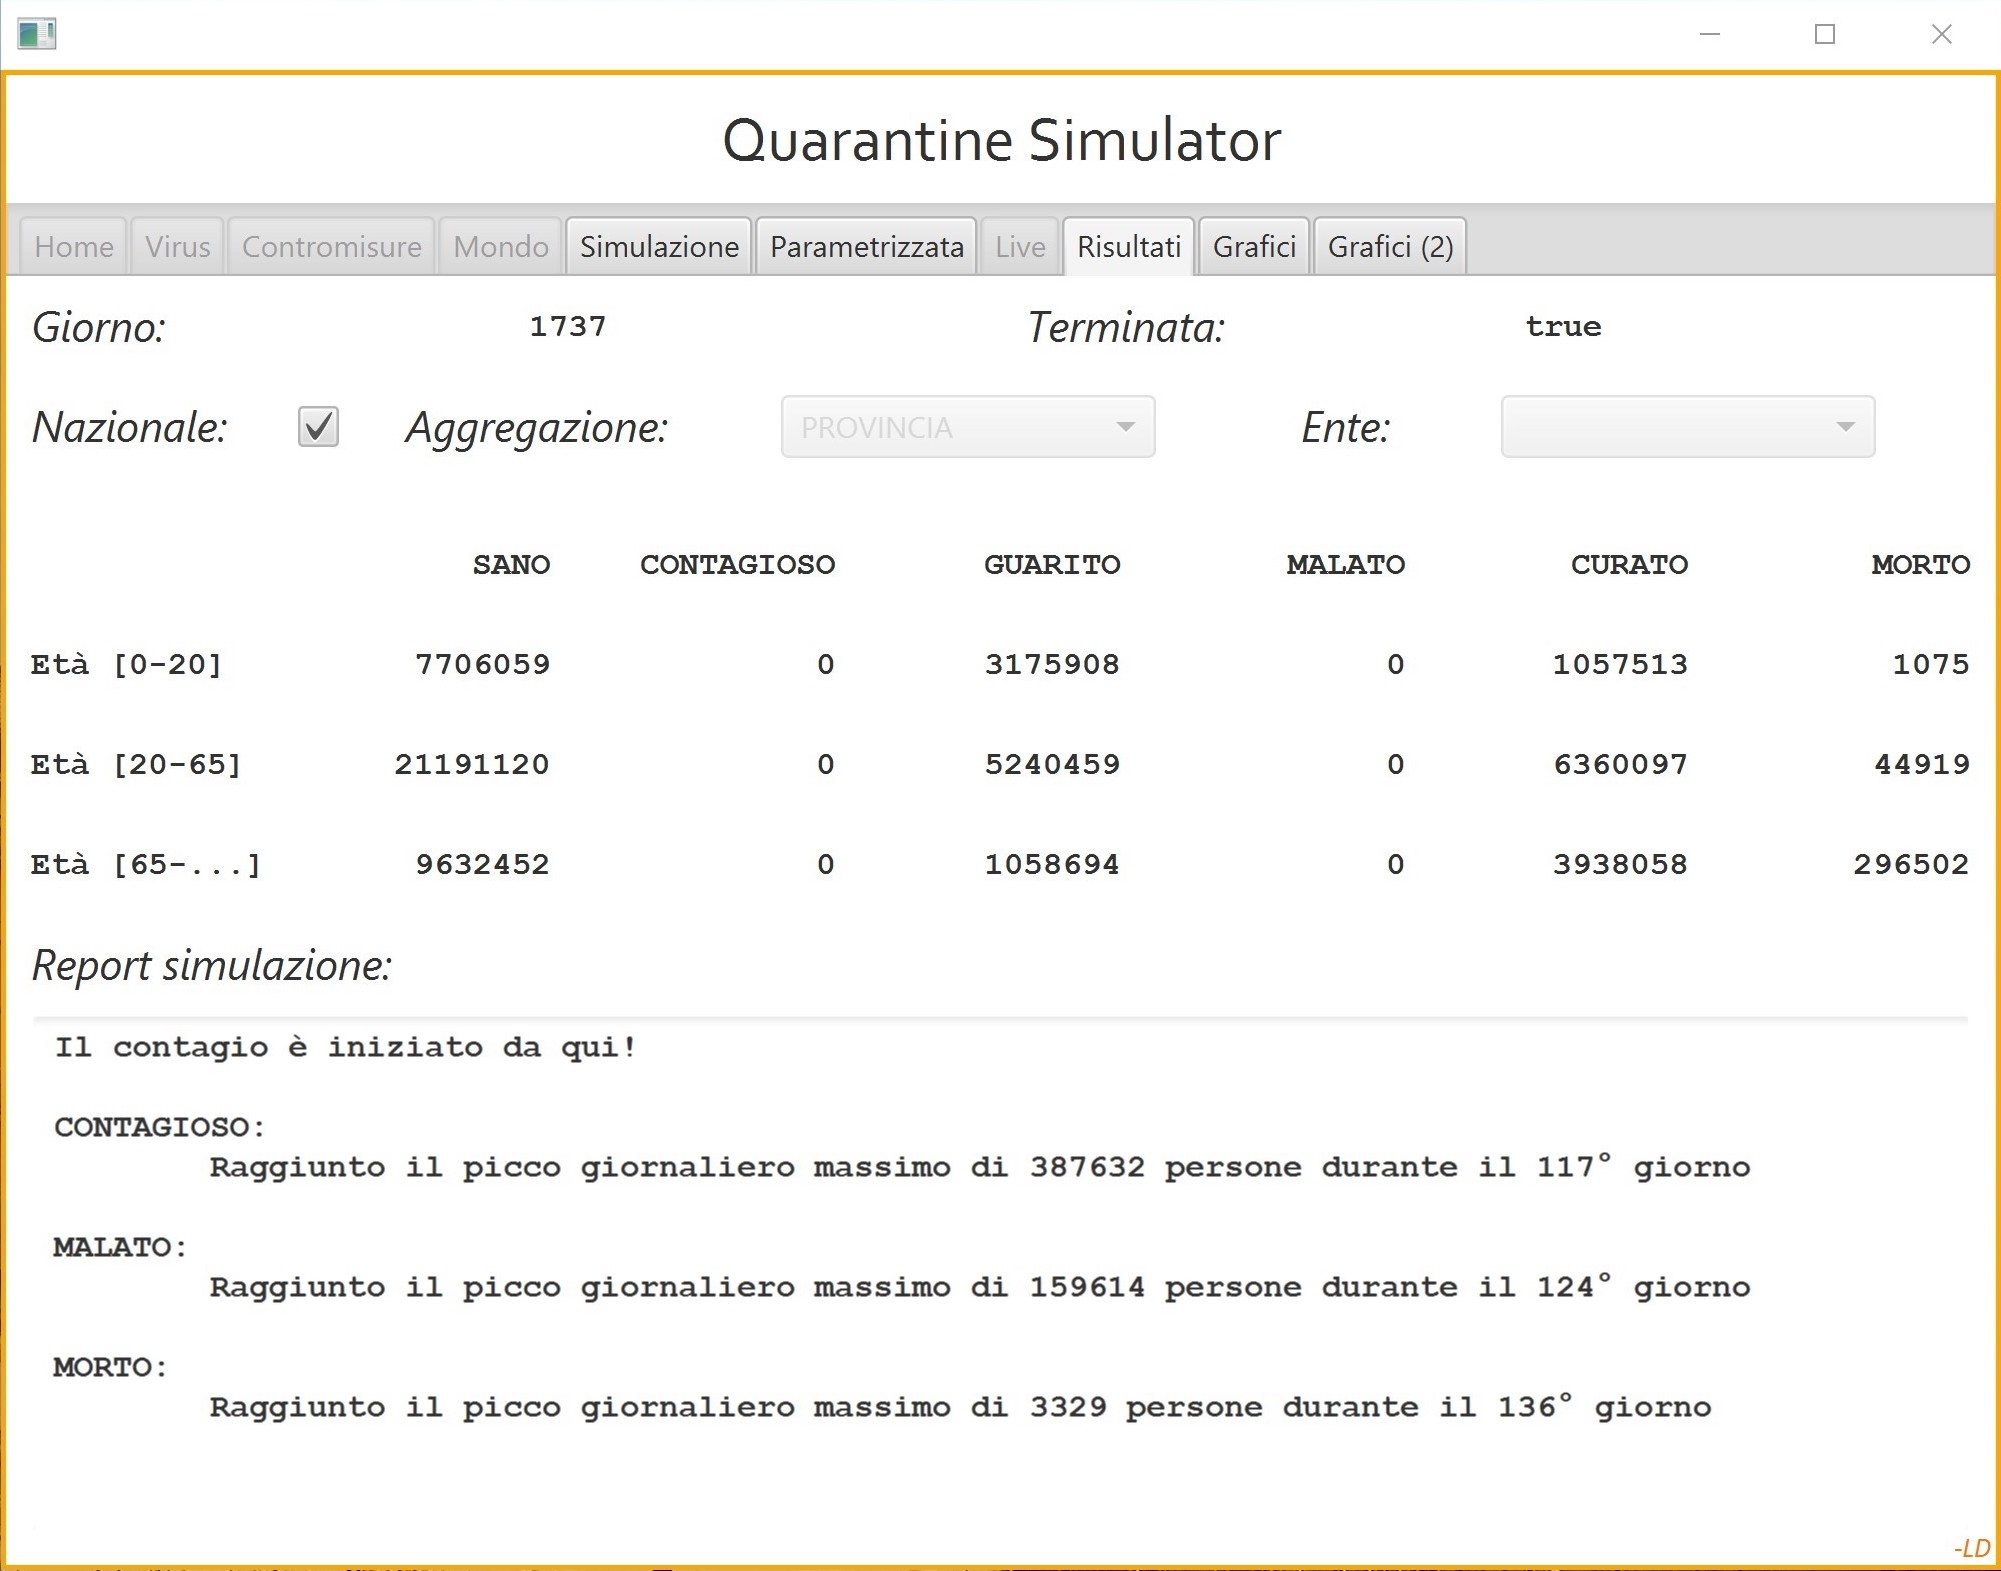
\includegraphics[height=0.4\textheight]{IMG/3.jpg}
	\caption[App: Tab Risultati]{Tab che contiene i risultati in formato tabellare. Qui sono mostrati a livello nazionale, ma il target può essere modificato a piacimento. Poiché l'epidemia non è stata gestita, il numero di vittime è elevatissimo.}
	\label{fig:screen3}
\end{figure}

\begin{figure}[H]
	\centering
	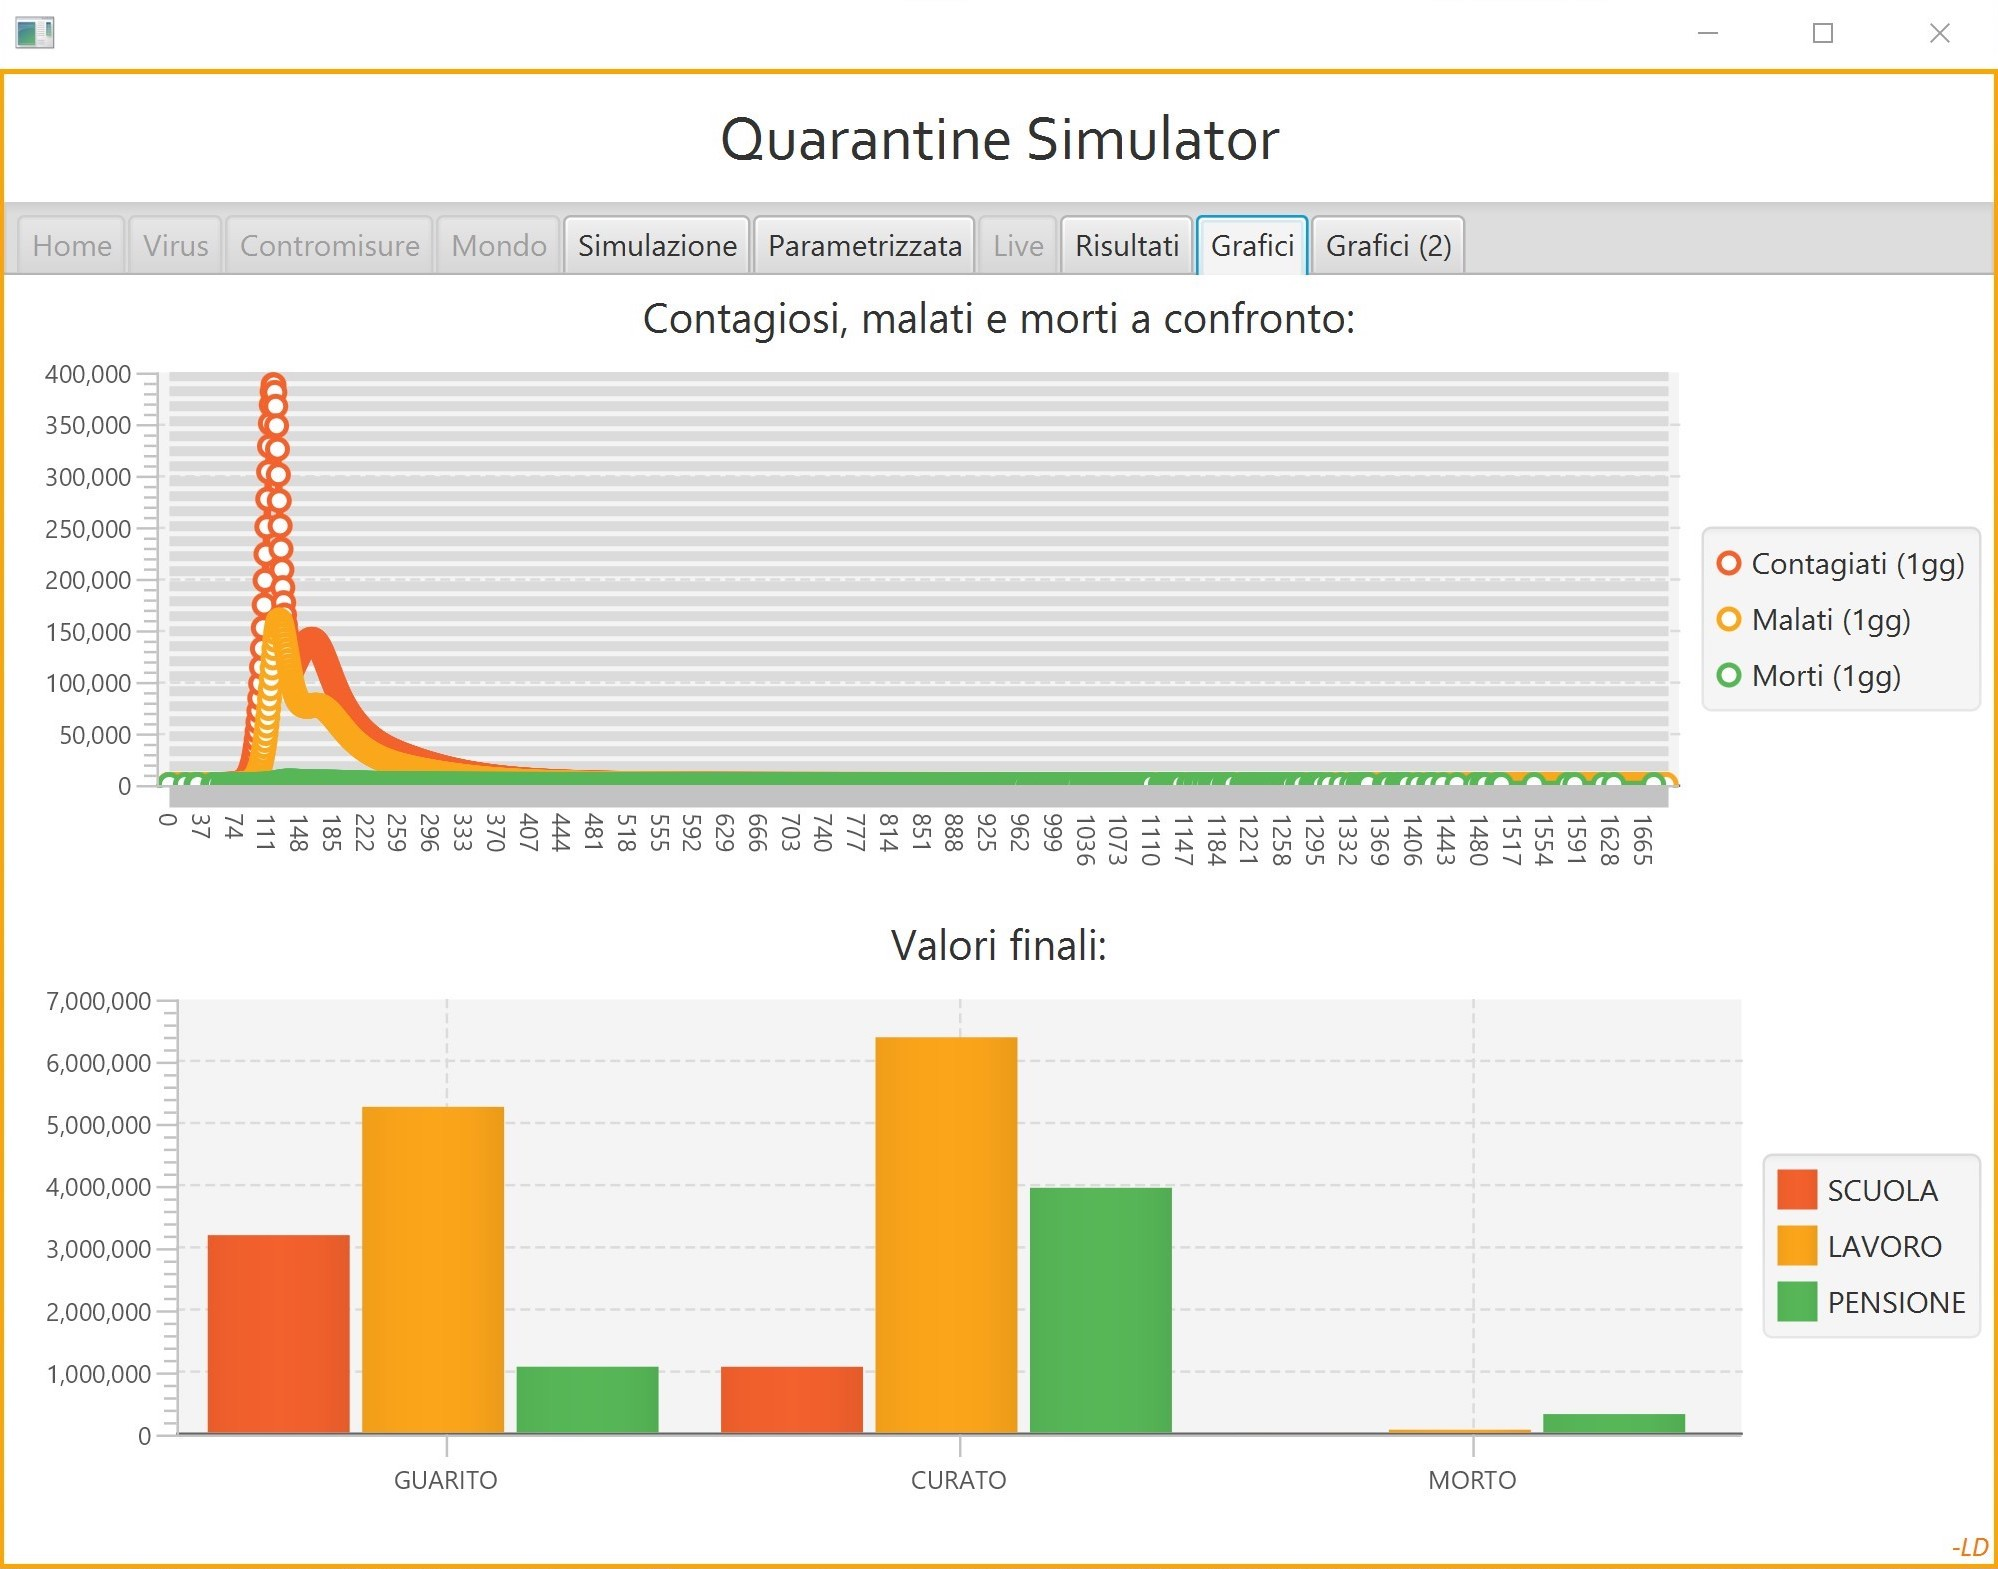
\includegraphics[height=0.4\textheight]{IMG/4.jpg}
	\caption[App: Tab Grafici (1)]{Grafici relativi all'ente selezionato in precedenza. Da essi risulta che la gran parte dei contagi è avvenuta durante il primo anno. Questo perché il virus è stato lasciato totalmente libero di espandersi, senza che nessuna misura atta ad ostacolarlo fosse presa.}
	\label{fig:screen4}
\end{figure}

\begin{figure}[H]
	\centering
	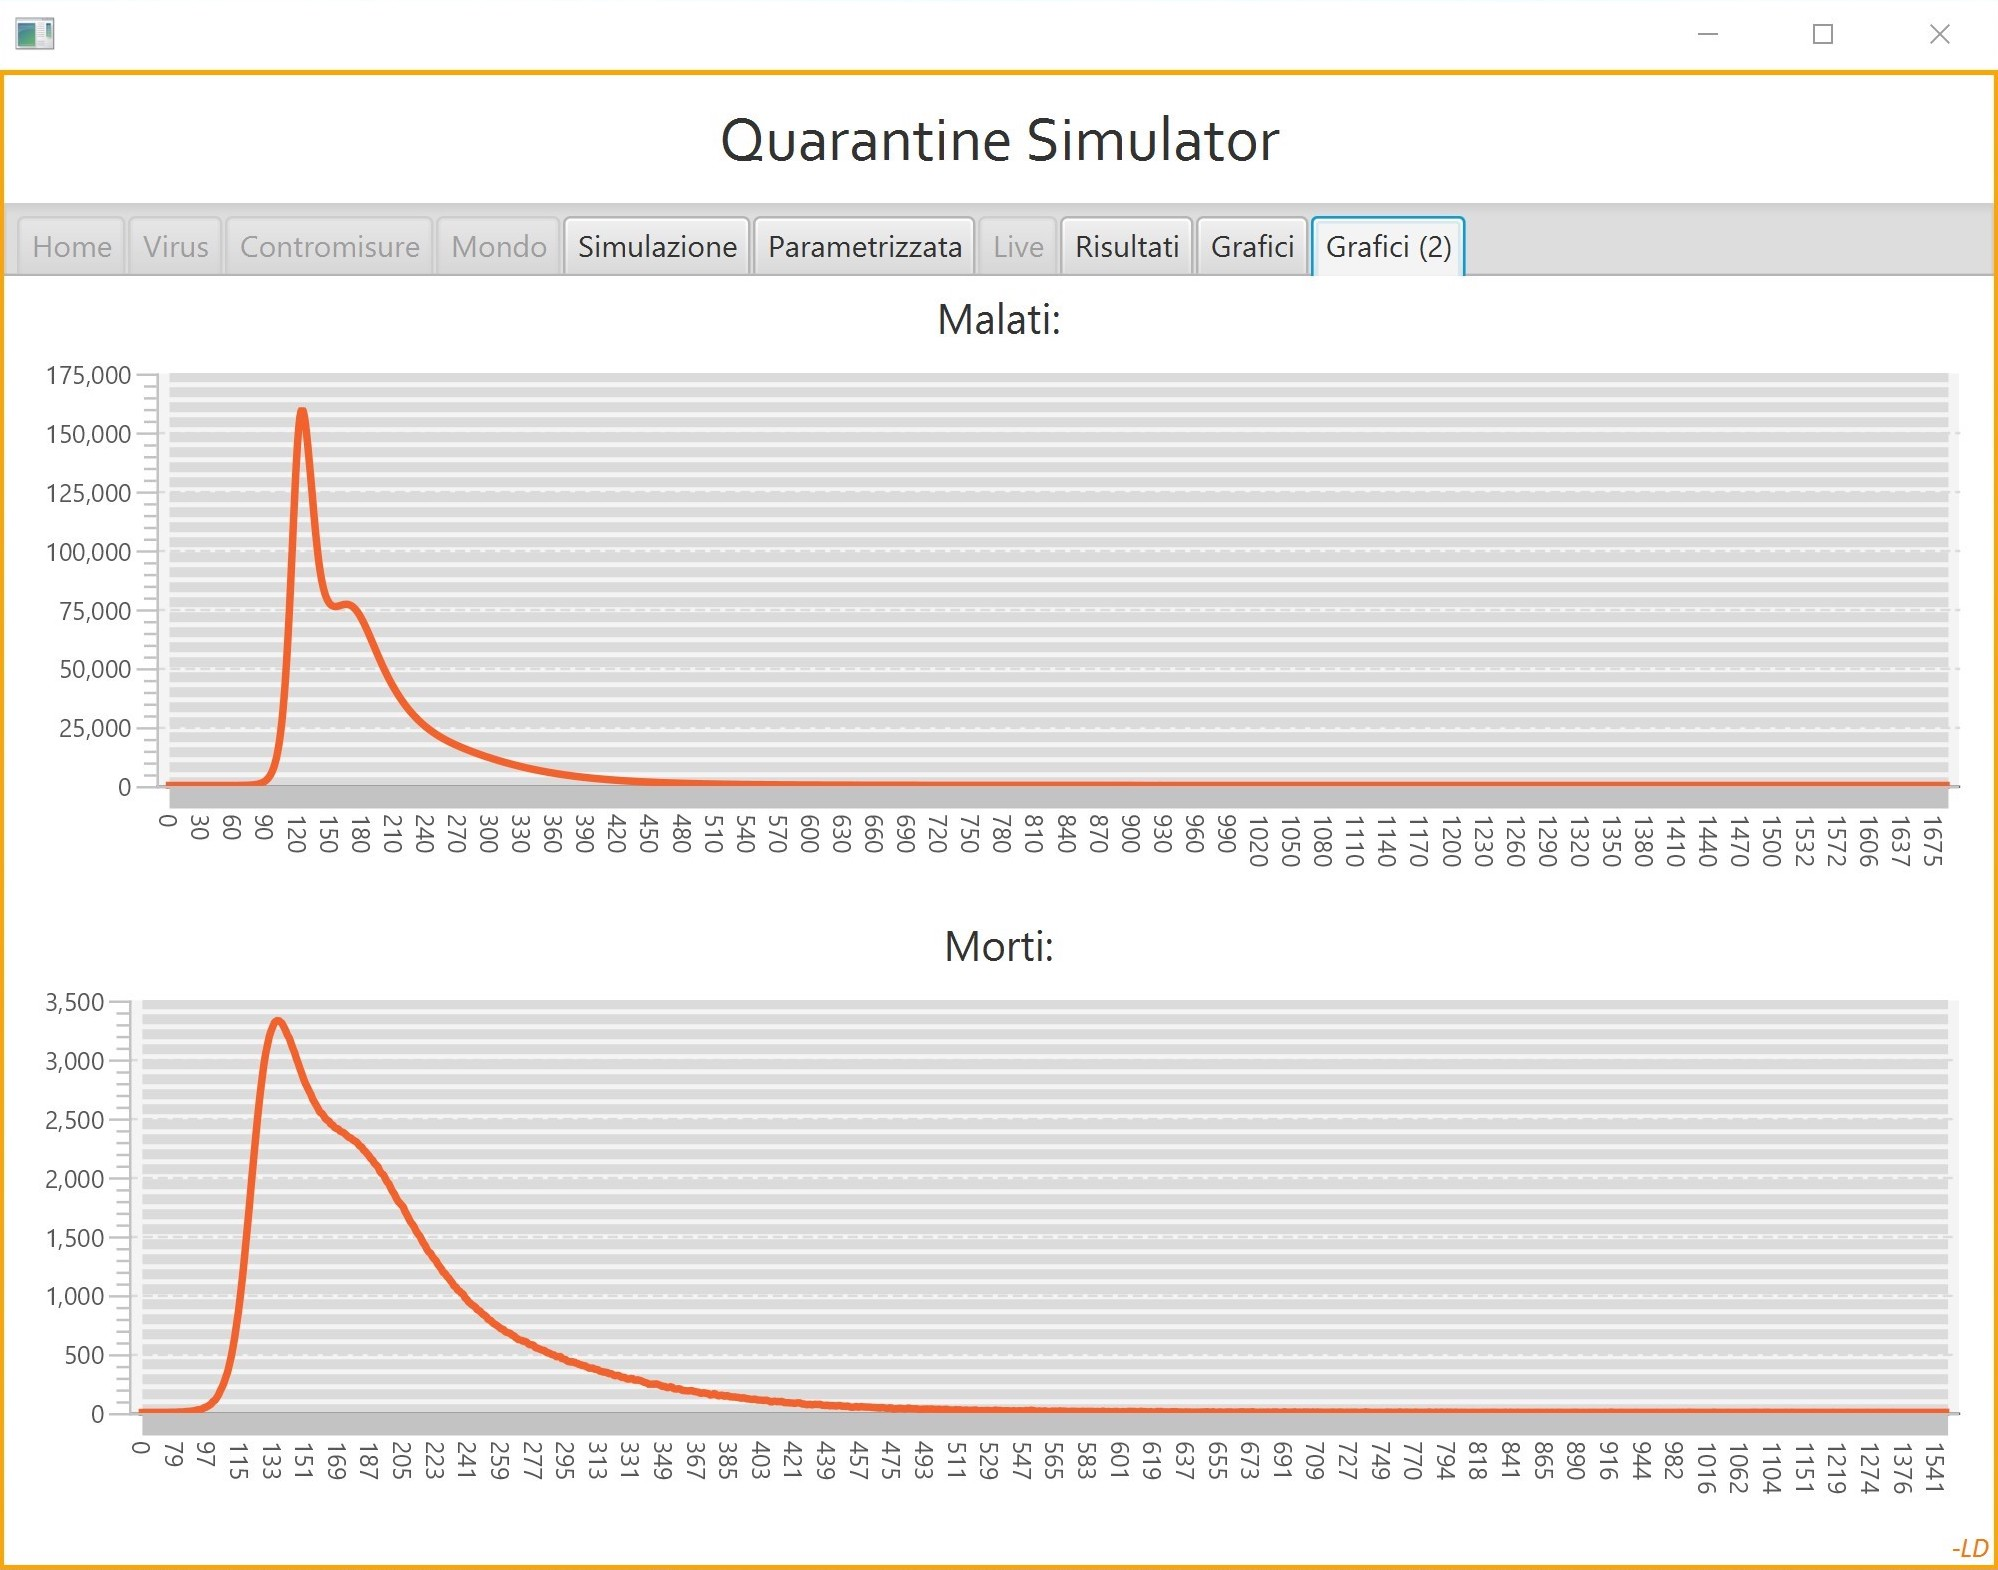
\includegraphics[height=0.4\textheight]{IMG/5.jpg}
	\caption[App: Tab Grafici (2)]{Continuazione dei grafici.}
	\label{fig:screen5}
\end{figure}
		
\newpage
% FUTURO

\section{Futuro}
	\label{sec:fut}
	Personalmente mi ritengo già estremamente soddisfatto del risultato ottenuto; sono tuttavia presenti numerose possibilità per ampliare e arricchire questo progetto.\\
	Ecco alcuni degli aspetti che sarebbe interessante approfondire:
	
	\begin{itemize}
		\item Coinvolgere in prima persona un epidemiologo, in modo da avere suggerimenti su come affinare l'algoritmo di evoluzione.
		\item Modellare la possibilità di importare nuovi contagiati dall'estero, magari come probabilità che, nei comuni di frontiera o in quelli dotati di grandi aeroporti, si sviluppi dal nulla un contagio.
		\item Inserire la possibilità di creare un vaccino che, aggiungendo un nuovo status e la logica che lo regola, permetta di trasformare ogni giorno un numero prefissato di persone dallo status di SANO a quello di VACCINATO.
		\item Rendere più evoluto il modello epidemiologico, magari trasformandolo dal semplice SIR al più complesso MSEIS.
		\begin{itemize}
			\item Persone con immunità naturale (M), che non possono prendere il virus e che quindi non contano come sani (ma che generano comunque contatti non a rischio).
			\item Aggiungere lo status di ESPOSTO (E), dove il virus è in incubazione e quindi il soggetto è sia asintomatico che non contagioso (da collocare come stato intermedio tra SANO e CONTAGIOSO).
			\item Rendere le persone guarite non immuni a vita e quindi di nuovo contagiabili (non più $\dots{}$R (Rimossi) ma $\dots{}$S (Suscettibili)).
			Questo è attuabile facendo in modo che, dagli stati di GUARITO e MALATO, sia possibile tornare a quello di SANO dopo un tempo medio di $t$ giorni.
		\end{itemize}
		Suddividere lo status MALATO in sottocategorie più specifiche, come ad esempio una che modella la quarantena in casa e un'altra l'ospedalizzazione.
		\item Specificare ulteriormente il punto precedente, suddividendo il ricovero in ospedale in vari livelli di gravità (LEGGERO, MEDIO, GRAVE).
		\item Aggiungere il numero di terapie intensive (o come db con valori puntuali, o anche solo come singolo valore nazionale) e regolare il tasso di mortalità degli individui nello stato di GRAVE sulla base della presenza o meno di posti liberi.
		\item Aggiungere un sistema di screening, che permetta di rimuovere alcuni soggetti contagiati prima che mostrino i sintomi.
		\item Inserire considerazioni di carattere economico, magari come perdite di PIL calcolate in funzione del protrarsi delle misure di quarantena e del numero di vittime e malati.
	\end{itemize}


\newpage
% BIBLIOGRAFIA
	
	\begin{thebibliography}{9}
		\bibitem{tes:LaTeX} Lorenzo Pantieri e Tommaso Gordini. \emph{L'arte di scrivere con \LaTeX}. 2019. URI: \url{http://www.lorenzopantieri.net/LaTeX_files/ArteLaTeX.pdf}.
		
		\bibitem{vir:mod} Matilde Italiano. \emph{Coronavirus: il modello matematico che ne descrive l’evoluzione}. 09/03/2020. URI: \url{https://sciencecue.it/coronavirus-modello-matematico-evoluzione/18355/}.
		
		\bibitem{vir:asint} Cristina Marrone su Corriere della Sera. \emph{Gli asintomatici sono contagiosi? Ecco cosa dice la scienza}. 10/06/2020. URI: \url{https://www.corriere.it/salute/malattie_infettive/}.
		
		\bibitem{vir:oms} World Health Organization. \emph{WHO Coronavirus Disease (COVID-19) Dashboard}. 2020. URI: \url{https://covid19.who.int/}.
		
		\bibitem{vir:sir} B. Cifra, L. Lamberti, S. Marone. \emph{SIR: un modello matematico di epidemie}. 2008-2009. URI: \url{https://dipmat.univpm.it/~demeio/public/Analisi_Numerica/sir.pdf}.
	\end{thebibliography}
	
	\vfill
	
	\begin{description}
		\centering
		\item[Repository:] \hfill \url{https://github.com/TdP-prove-finali/DebernardiLuca}
		\item[Video informativo:] \hfill \url{https://youtu.be/bRDcXdKuuVo}
	\end{description}

\newpage
% LICENZA


	$\text{}$
	\vfill
	\centering
	\textbf{Quarantine Simulator} by Luca Debernardi\\ is licensed under CC BY-NC-SA 4.0. A copy of this license is available at \url{https://creativecommons.org/licenses/by-nc-sa/4.0}.
	
	\begin{center}
		
\includegraphics[width=0.45\textwidth]{IMG/CC-BY-NC-SA_icon.png}
	\end{center}
	
	
\end{document}